\chapter{Entwicklung des \gls{SoC}}
\label{cha:plasma_extension}

In diesem Kapitel wird die Entwicklung der \gls{SoC}-Komponenten und ihre Integration zum Plasma-\gls{SoC} beschrieben.

Bisher standen alle peripheren Geräte und Speicher durch manuelle Adresszuordnung dem Plasma zur Verfügung. Die Adressdekodierung und Verdrahtung aller Komponenten war im Ausgangsprojekt als ein weiterer Prozess in der Datei \textit{plasma.vhd} umgesetzt. Jegliche Erweiterung erforderte eine händische Anpassung der Adressdekoder sowie der Anbindung zusätzlicher Register. Dieses Verfahren funktioniert nur so lange gut, wie es wenige anzubindende Geräte mit niedriger Komplexität gibt. 

Bei vielen Komponenten, die hinzuzufügen wären, würde die Übersicht sehr schnell verloren gehen. Zudem müssen die Komponenten von Hand miteinander verbunden werden und der Wartungsaufwand würde ins Unermessliche steigen. 

Im Rahmen der Veranstaltung \enquote{\subjectphv{}} wurde bereits ein rudimentäres Bussystem entwickelt, welches sich jedoch aufgrund von Fehlern und Nichtkonformität als ungeeignet erwies. Darum wurde der in \cref{the:bus_system} beschriebene Wishbone Bus umgesetzt.

\section{Komponenten}
\label{sec:plasma_soc_components}
Für die bereits vorhandenen Komponente wie die Plasma-CPU, \gls{RAM}, \gls{UART}, etc. wurden Wishbone-Schnittstellen entwickelt. Außerdem müssen viele neue Komponenten neu entwickelt werden, um das zugrundeliegende Plasma-System zu einem benutzbaren eingebetteten System auszubauen. Diese wurden ebenfalls zweiteilig entwickelt: Modul-Logik ist von der Schnittstellen-Logik getrennt. Zu diesen gehören der Interrupt-Controller, Zähler, Timer,\gls{GPIO}-, \gls{UART}-, \gls{SPI}-Schnittstellen sowie der Display-Controller.


\begin{table}[!htbp]
	\bigskip
	\centering
	\begin{tabular}{  l | r | r | l }
		\textbf{REGISTER} & \textbf{Adresse} & \textbf{Modus} & \textbf{Beschreibung} \\
		\hline
		control & 0x00 & r/w & control register (reserved)\\
		status & 0x04 & r & status register (reserved)\\
		data & 0x08 & r/w & data register (reserved)\\
		\vdots & \vdots & \vdots & user defined \\
		\hline		
		\textbf{CONTROL-Register} & \textbf{Bit} & & \\
		\hline
		reset & 0 & r/w & reset device (reserved)\\
		enable & 1 & r/w & enable device (reserved)\\
		\vdots & \vdots & \vdots & user defined \\
		\hline		
		\textbf{STATUS-Register} & \textbf{Bit} & & \\
		\hline
		ready & 0 & r & device ready (reserved)\\
		davail & 1 & r & data available (reserved)\\
		\vdots & \vdots & \vdots & user defined \\
		\hline
	\end{tabular}
	
	\caption{Konsolidiertes Register- und Flagschema}
	\label{tab:device_reg_map}
\end{table}

Es wurde ein einheitliches Register- und Flagschema für alle Wishbone-Slaves entworfen (siehe \cref{tab:device_reg_map}). An den unteren drei Adressen liegen nacheinander das Kontroll-, Status- und Datenregister. Zudem sind die unteren Bits der Kontroll- und Statusregister reserviert. Alle benutzerdefinierten Register und Flags sind nach den reservierten einzutragen. Durch diese Vereinheitlichung vereinfacht sich sowohl die Geräte- als auch die Treiberentwicklung. Selbstverständlich kann dieses Schema für Komponenten von Drittanbietern nicht erwartet werden.

\subsection{CPU}

\begin{figure}[!htbp]
	\centering
	
\includegraphics[width=0.3\linewidth]{images/cpu}
	\caption{Schaltplanausschnitt: CPU Master}
	\label{fig:shared_bus_master_cpu_sch}
\end{figure}

Der Plasma Prozessor musste wie alle anderen Komponenten an das Wishbone-Interface angepasst werden. Um destruktive Änderungen an der Komponente zu vermeiden, fiel die Entscheidung auf einen Wishbone-Wrapper als zusätzliche Entität. Der Wrapper kontrolliert die \textit{cyc} und \textit{stb} Ausgangssignale, und reagiert auf \textit{ack}, \textit{stall}, \textit{err}, \textit{rty} Signale. 

\subsection{RAM (Intern)}
\label{sec:internal_ram}
\begin{figure}[!htbp]
	\centering
	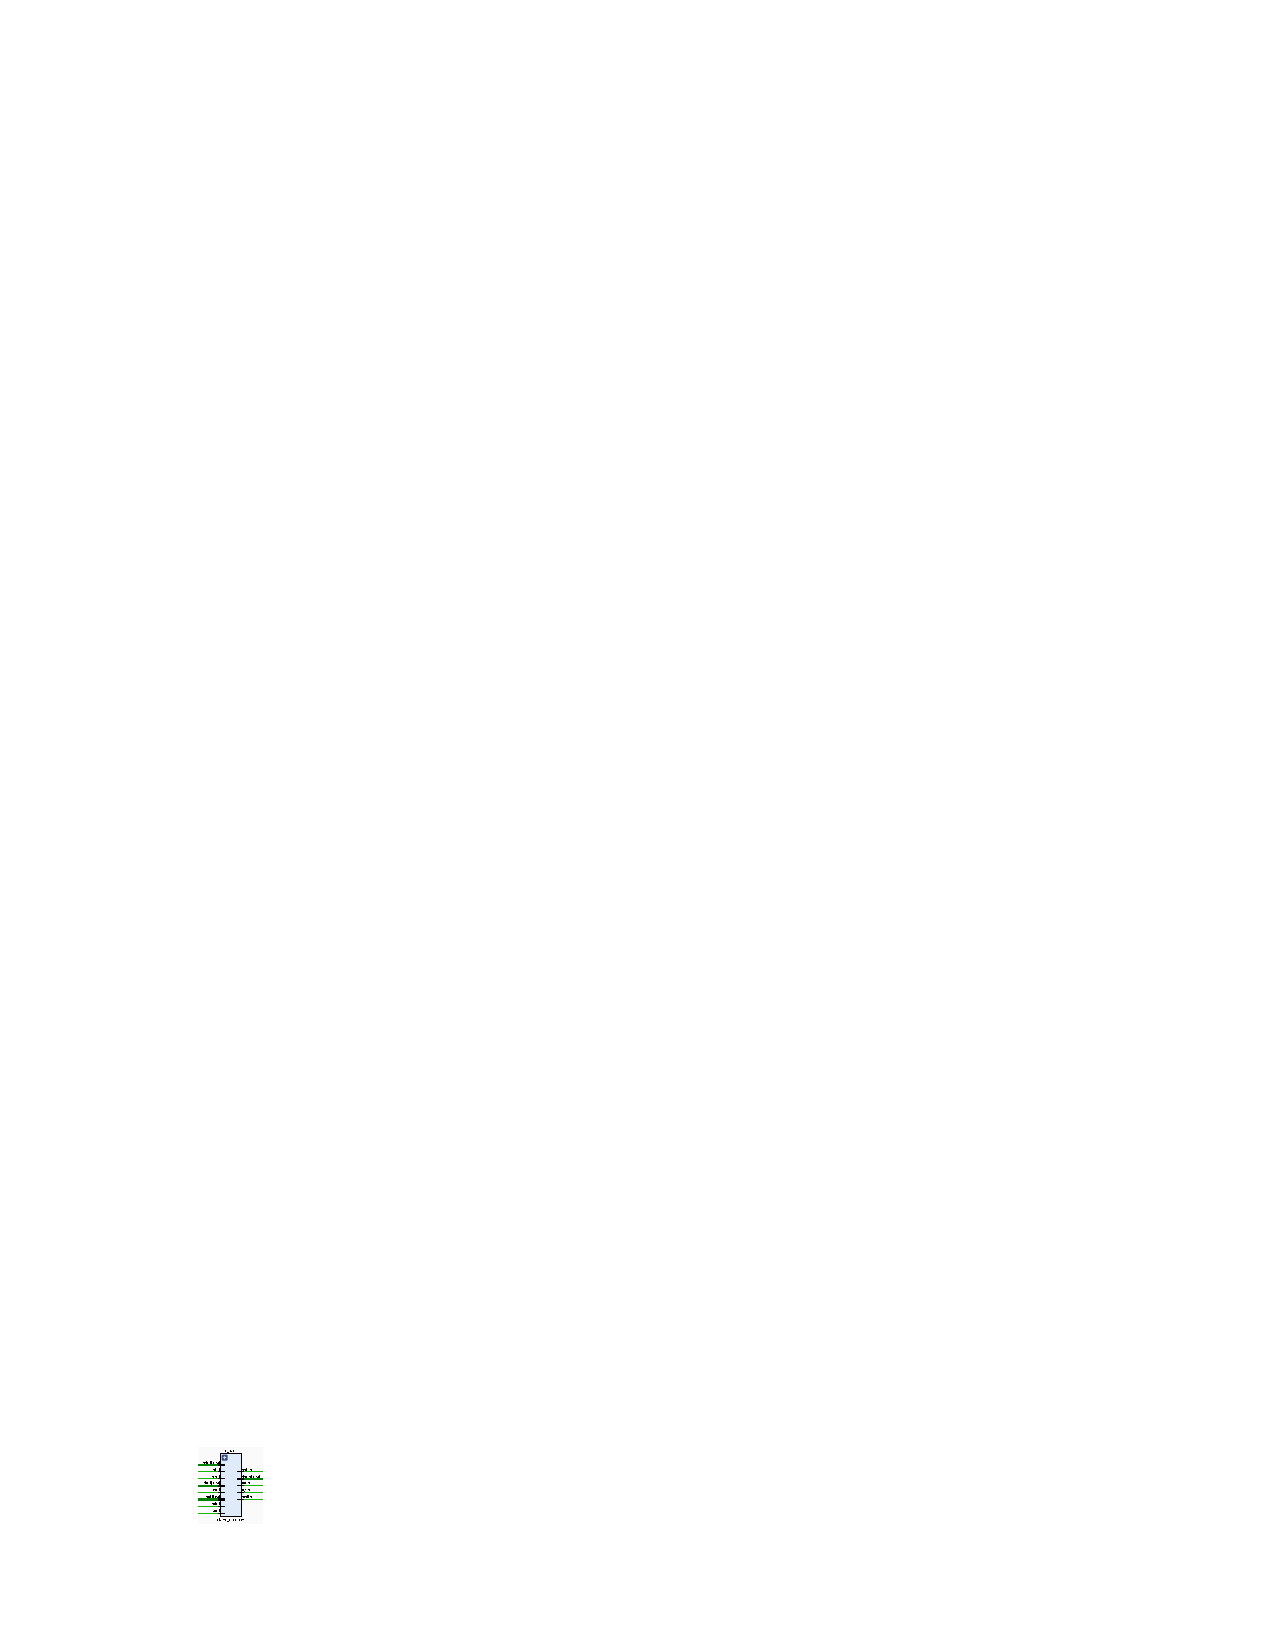
\includegraphics[width=0.3\linewidth]{images/ram}
	\caption{Schaltplanausschnitt: RAM Slave}
	\label{fig:shared_bus_ram_sch}
\end{figure}

Der RAM muss ebenfalls an den Wishbone Bus angebunden werden. Der entsprechende Wrapper ist im Vergleich zu anderen Devices sehr einfach, da das in \cref{tab:device_reg_map} beschriebene Schema hier nicht befolgt werden muss.

\subsection{RAM (Extern)}

\begin{figure}[!htbp]
	\centering
	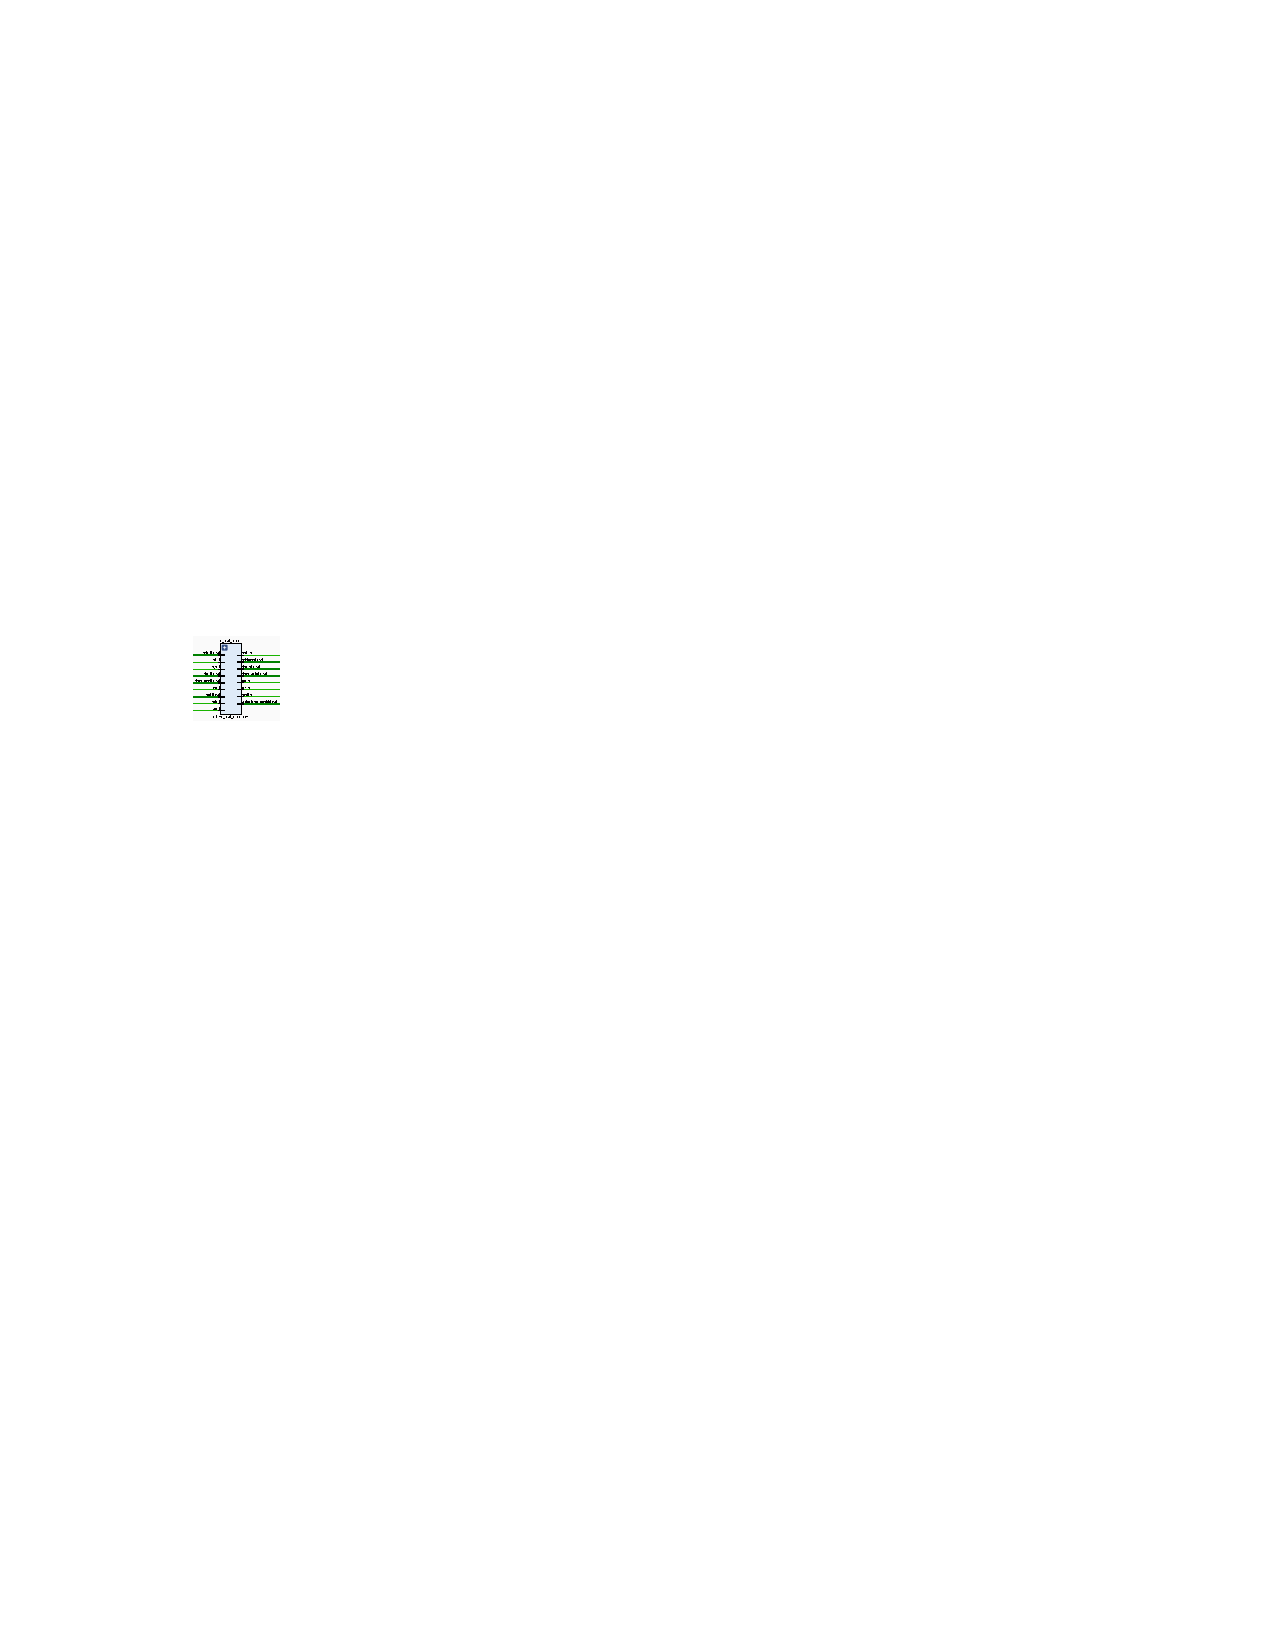
\includegraphics[width=0.3\linewidth]{images/ext_mem}
	\caption{Schaltplanausschnitt: Externer RAM Slave}
	\label{fig:shared_bus_ext_mem_sch}
\end{figure}

Der externe RAM ist als Dummy-Wrapper umgesetzt. Im Wrapper wird kein RAM-Controller instanziiert. Ebenso wird, wie in \cref{sec:internal_ram} bereits erwähnt, das Registerschema nicht befolgt.

\subsection{Interrupt Controller}

Der Interrupt Controller wurde aus P. Tofahrns Abschlussprojekt \cite{article:plasma_interrupt_controller} übernommen und angepasst. Für diesen wurde ebenfalls ein Wishbone-Wrapper entwickelt. Zusätzlich waren Änderungen an der Plasma-CPU notwendig, da die CPU \textquote{bei einem Reset an Adresse 0 und bei einem Interrupt an 0x3C} \cite[5]{article:plasma_interrupt_controller} sprang.

\begin{figure}[!htbp]
	\centering
	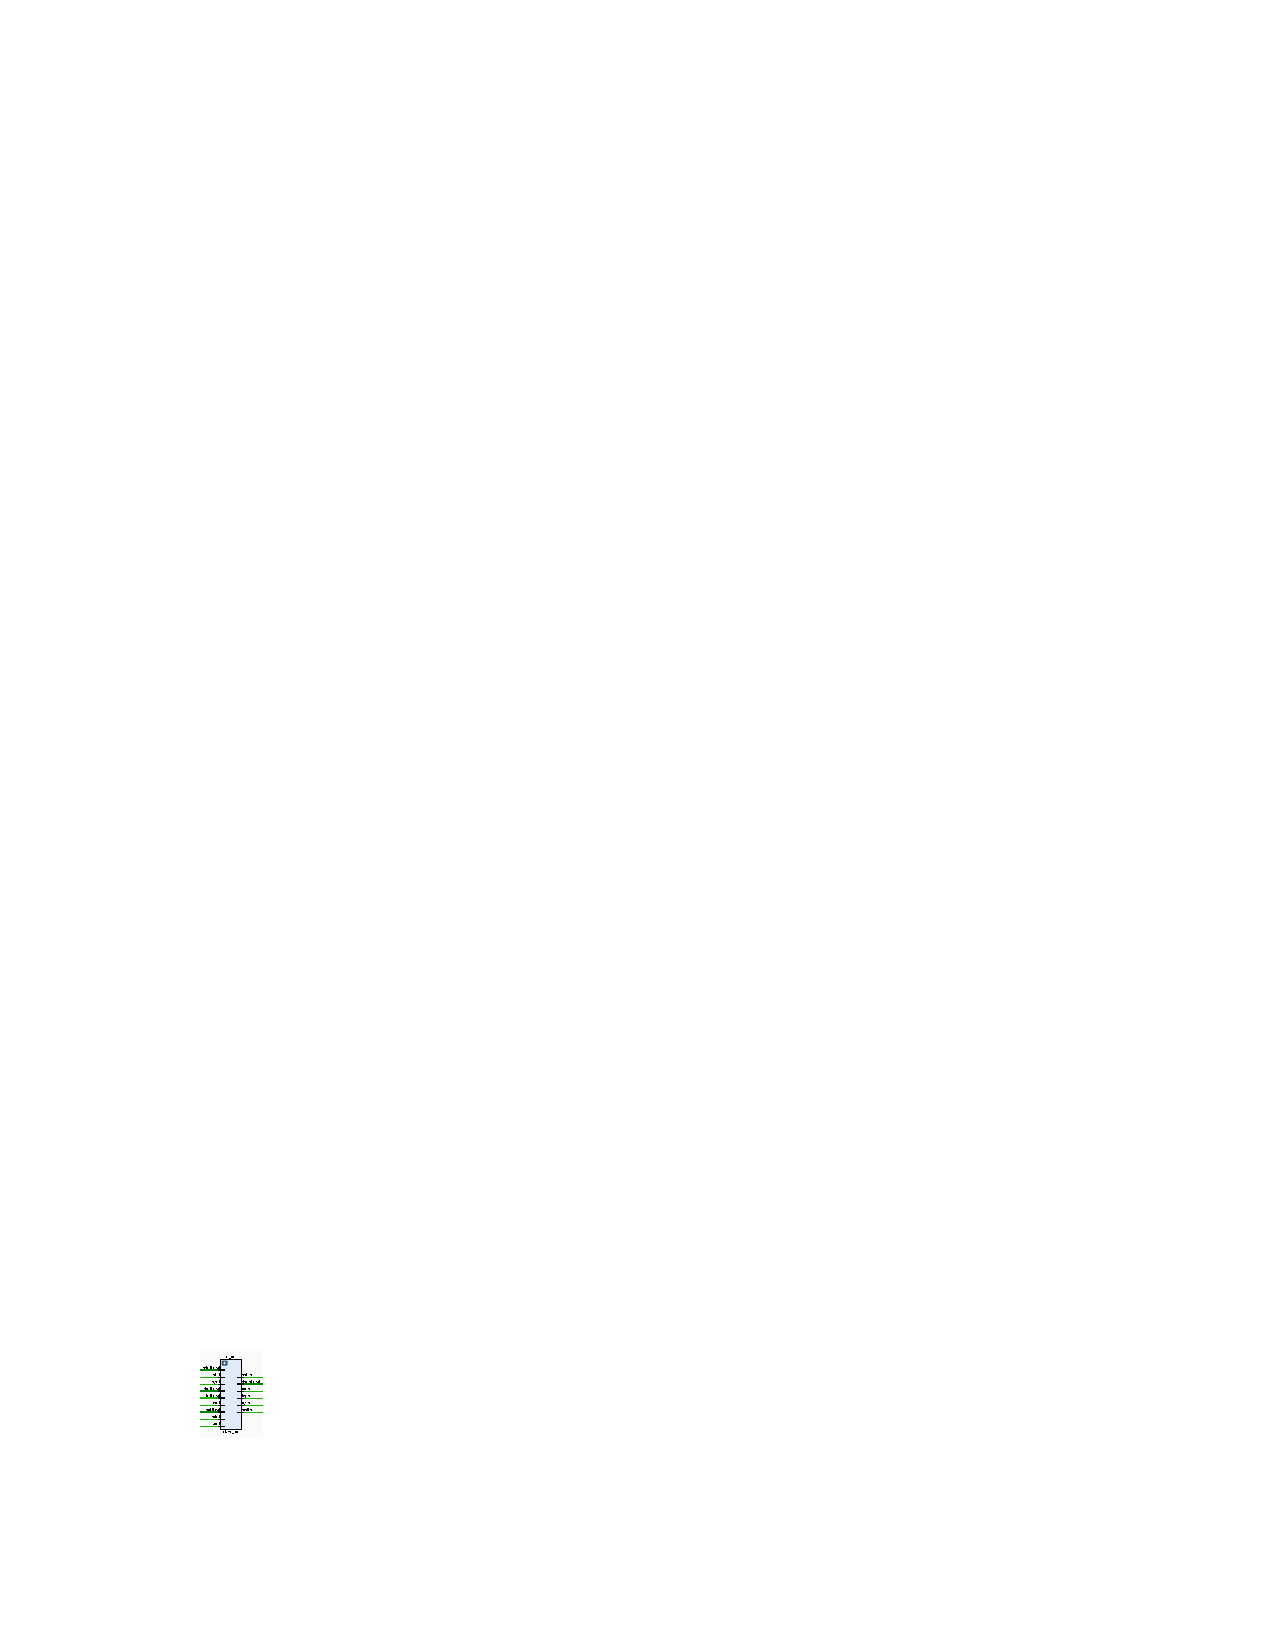
\includegraphics[width=0.3\linewidth]{images/irc}
	\caption{Schaltplanausschnitt: Interrupt Controller Slave}
	\label{fig:shared_bus_irc_sch}
\end{figure}

\begin{table}[!htbp]
	\bigskip
	\centering
	\begin{tabular}{  l | r | r | l }
		\textbf{REGISTER} & \textbf{Adresse} & \textbf{Modus} & \textbf{Beschreibung} \\
		\hline
		control & 0x00 & r/w & control register \\
		status & 0x04 & r/w & status register \\
		data & 0x08 & r & interrupt flag state \\
		imm flags & 0x0C & r & immediate interrupt flag state \\
		clear & 0x10 & r/w & clear interrupt flag \\
		invert & 0x14 & r/w & interrupt polarity\\
		mask & 0x18 & r/w & interrupt flag enable/disable mask \\
		mask & 0x1C & r/w & interrupt edge detection \\
		\hline		
		\textbf{CONTROL-Register} & \textbf{Bit} & & \\
		\hline
		reset & 0 & r/w & reset device \\
		enable & 1 & r/w & enable device \\
		\hline		
		\textbf{STATUS-Register} & \textbf{Bit} & & \\
		\hline
		ready & 0 & r & device ready \\
		\hline
	\end{tabular}
	
	\caption{Registermapping Interrupt Controller}
	\label{tab:ir_contrroller_reg_map}
\end{table}

\subsection{Zähler}

\begin{figure}[!htbp]
	\centering
	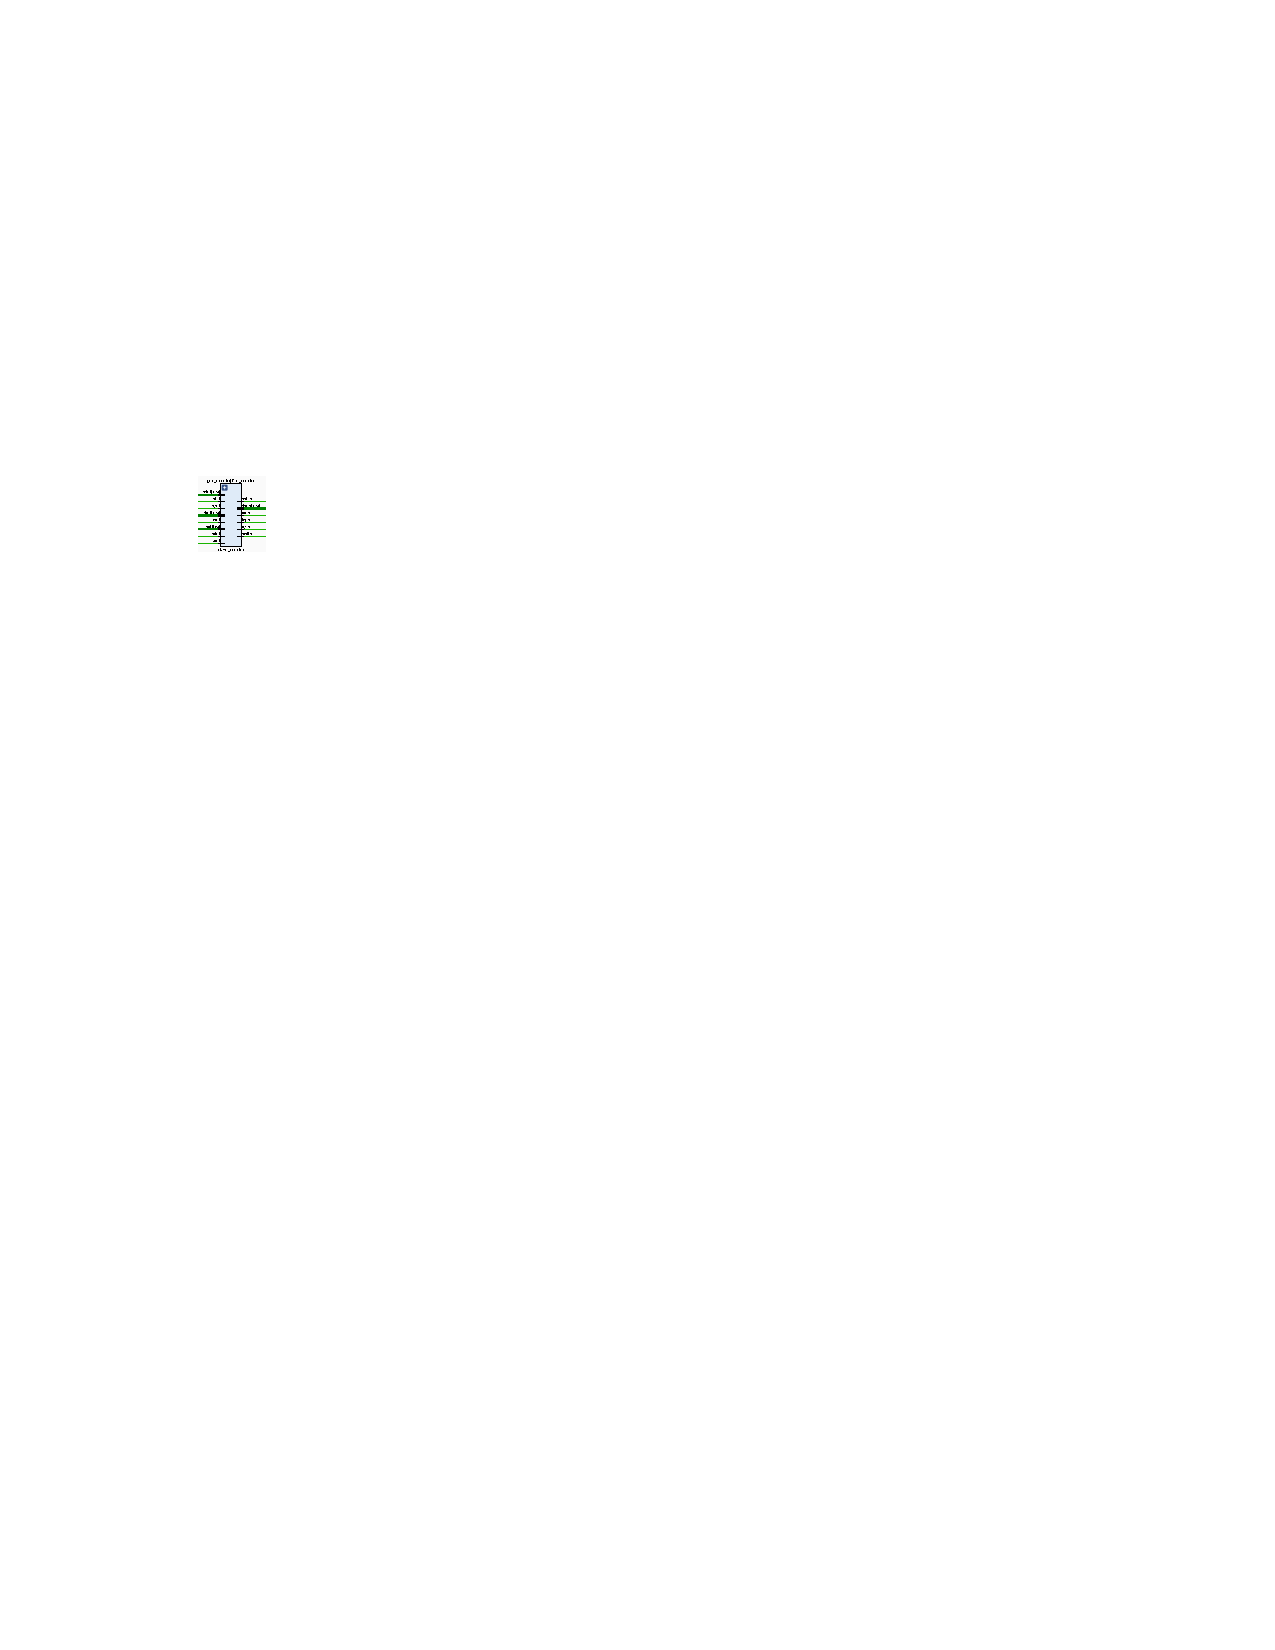
\includegraphics[width=0.3\linewidth]{images/counter}
	\caption{Schaltplanausschnitt: Zähler}
	\label{fig:shared_bus_counter_sch}
\end{figure}

Es wurde eine Zähler-Komponente entwickelt. Konfigurierbar sind die Zählerrichtung, Reload-Wert sowie der Auto-Reload (Beim Überlauf wird automatisch zurückgesetzt und neu gezählt). Bei Erreichen eines Grenzwertes (Aufwärts: ReloadValue - 1, Abwärts: 0) wird ein Interrupt ausgelöst. Details sind in \cref{tab:counter_reg_map} dargestellt.

\begin{table}[!htbp]
	\bigskip
	\centering
	\begin{tabular}{  l | r | r | l }
		\textbf{REGISTER} & \textbf{Adresse} & \textbf{Modus} & \textbf{Beschreibung} \\
		\hline
		control & 0x00 & r/w & control register \\
		status & 0x04 & r/w & status register \\
		data & 0x08 & r/w & data register (current counter value) \\
		reload & 0x0C & r/w & reload value \\
		\hline		
		\textbf{CONTROL-Register} & \textbf{Bit} & & \\
		\hline
		reset & 0 & r/w & reset device \\
		enable & 1 & r/w & enable device \\
		autoreload & 2 & r/w & reload on overflow \\
		direction & 3 & r/w & direction (0 = count up, 1 = count down) \\
		\hline		
		\textbf{STATUS-Register} & \textbf{Bit} & & \\
		\hline
		ready & 0 & r & device ready \\
		overflow & 1 & r & timer overflow \\
		\hline
	\end{tabular}
	
	\caption{Registermapping Zähler}
	\label{tab:counter_reg_map}
\end{table}

\subsection{Timer}
\label{ss:timer}

\begin{figure}[!htbp]
	\centering
	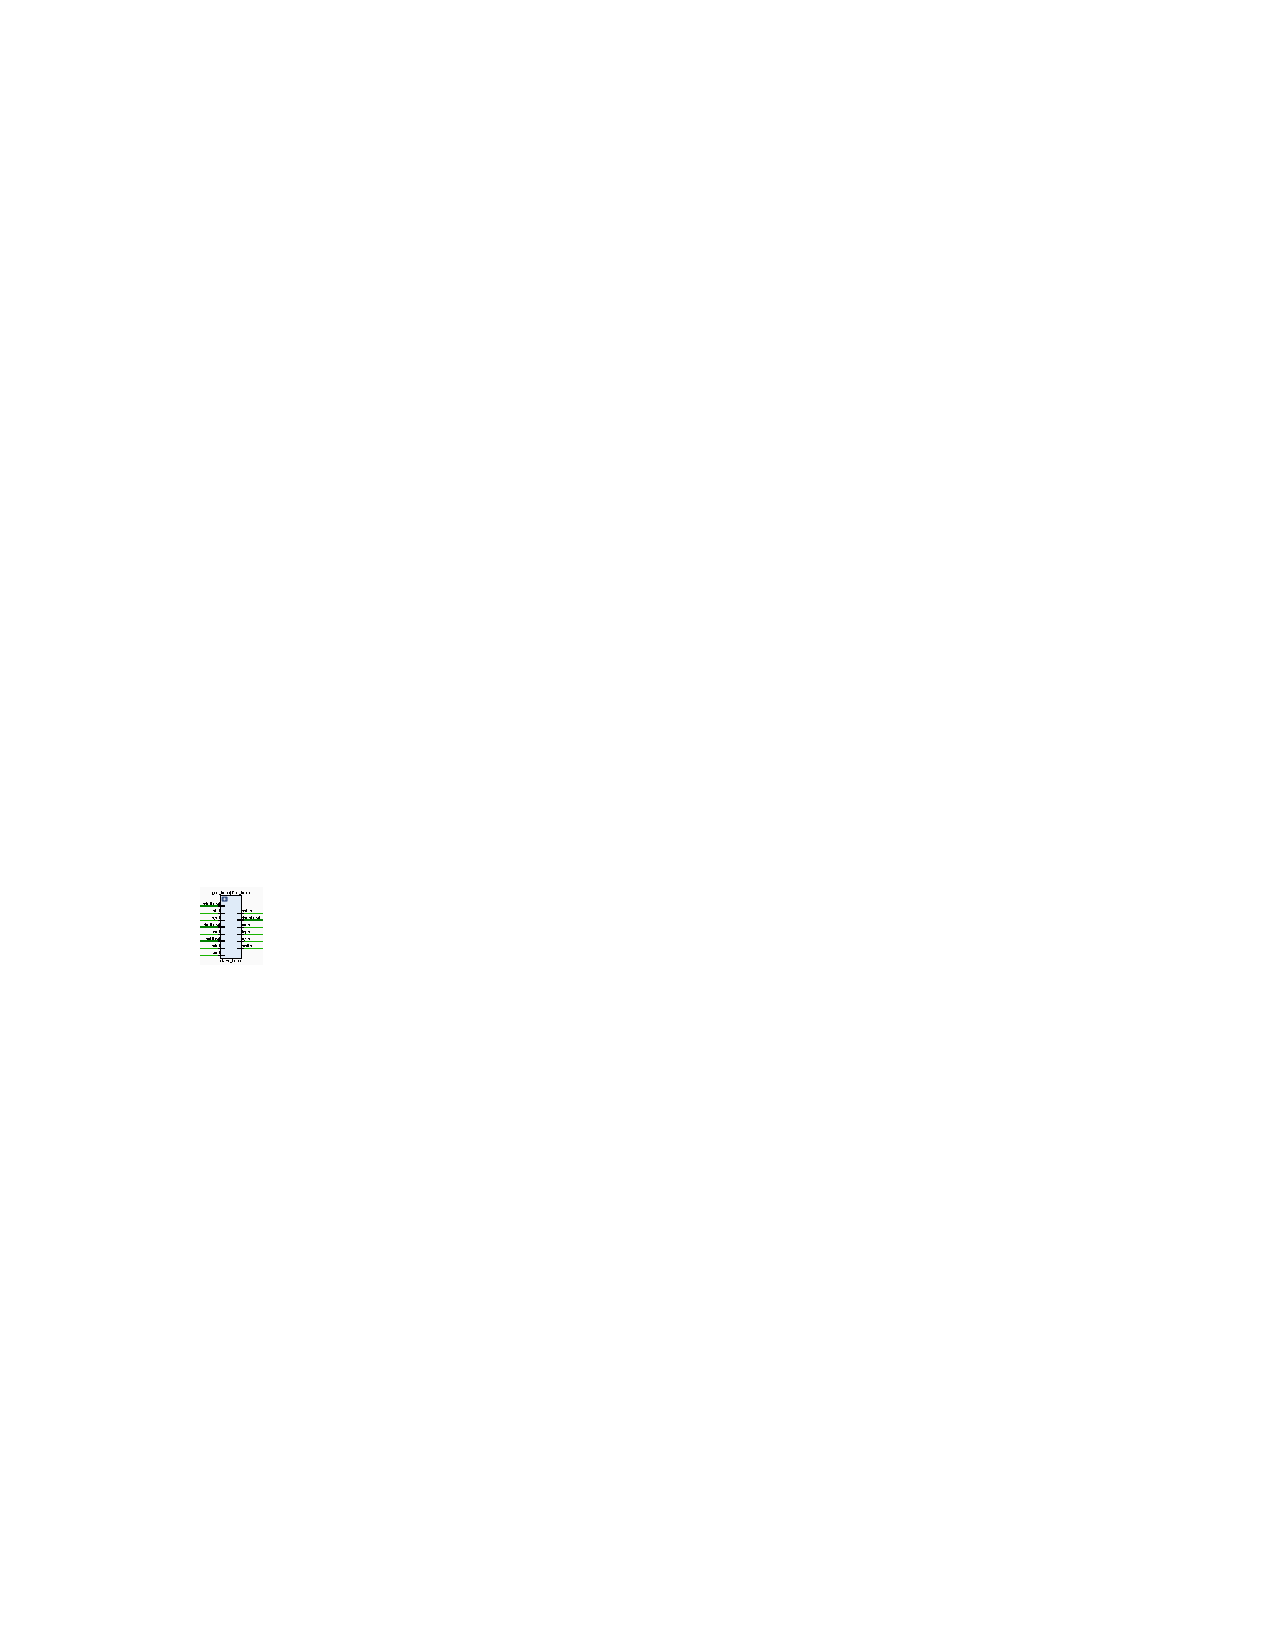
\includegraphics[width=0.3\linewidth]{images/timer}
	\caption{Schaltplanausschnitt: Timer}
	\label{fig:shared_bus_timer_sch}
\end{figure}

Die Timer-Komponente baut auf dem Zähler auf mit einem zeitlich angepasstem Reload-Wert, sodass die Zeit präzise gemessen werden kann. Die Werte für einen Systemtakt von $f_{sys} = \SI{50}{\mega\hertz}$ sind in \cref{tab:timer_units} aufgelistet. Die Grundeinheit ist $\SI{1}{\tick} = 1 = \frac{1}{T_{sys}} * f_{sys} | T_{sys} = \frac{1}{f_{sys}}$, was einem Taktzyklus entspricht.
Bei Erreichen des Schwellwertes wird - analog zum Zähler - ein Interrupt ausgelöst. Zudem lässt sich der Autoreset, so wie beim Zähler, konfigurieren.

\begin{table}[!htbp]
	\bigskip
	\centering
	\begin{tabular}{  l | r | r | l }
		UNIT & unit register value & reload value [ticks] \\
		\hline
		\SI{1}{\tick}  & 0 & $1$ & $  \frac{1}{T_{sys}} * f_{sys} = 1 $ \\
		\SI{1}{\nano\second} & 1 & $ 50 * 10^{-3} $ & $ f_{sys} * \SI{1}{\nano\second} = f_{sys} * \SI{1e-9}{\second} $ \\
		\SI{1}{\micro\second} & 2 & $ 50 * 10^0 $ & $ f_{sys} * \SI{1}{\micro\second} = f_{sys} * \SI{1e-6}{\second} $ \\
		\SI{1}{\milli\second} & 3 & $ 50 * 10^3 $ & $ f_{sys} * \SI{1}{\milli\second} = f_{sys} * \SI{1e-3}{\second} $ \\
		\SI{1}{\second} & 4 & $ 50 * 10^6 $  & $ f_{sys} * \SI{1}{\second} = f_{sys} * \SI{1e-0}{\second} $\\
		\hline
	\end{tabular}
	
	\caption{Timer einheiten}
	\label{tab:timer_units}
\end{table}

\begin{table}[!htbp]
	\bigskip
	\centering
	\begin{tabular}{  l | r | r | l }
		\textbf{REGISTER} & \textbf{Adresse} & \textbf{Modus} & \textbf{Beschreibung} \\
		\hline
		control & 0x00 & r/w & control register \\
		status & 0x04 & r/w & status register \\
		data & 0x08 & r/w & data register (current timer value) \\
		reload & 0x0C & r/w & reload value \\
		\hline		
		\textbf{CONTROL-Register} & \textbf{Bit} & & \\
		\hline
		reset & 0 & r/w & reset device \\
		enable & 1 & r/w & enable device \\
		autoreload & 2 & r/w & reload on overflow \\
		unit & 3:5 & r/w & timer time unit \\
		\hline		
		\textbf{STATUS-Register} & \textbf{Bit} & & \\
		\hline
		ready & 0 & r & device ready \\
		overflow & 1 & r & timer overflow \\
		\hline
	\end{tabular}
	
	\caption{Registermapping Timer}
	\label{tab:timer_reg_map}
\end{table}


\subsection{UART}
\label{ss:uart}
\begin{figure}[!htbp]
	\centering
	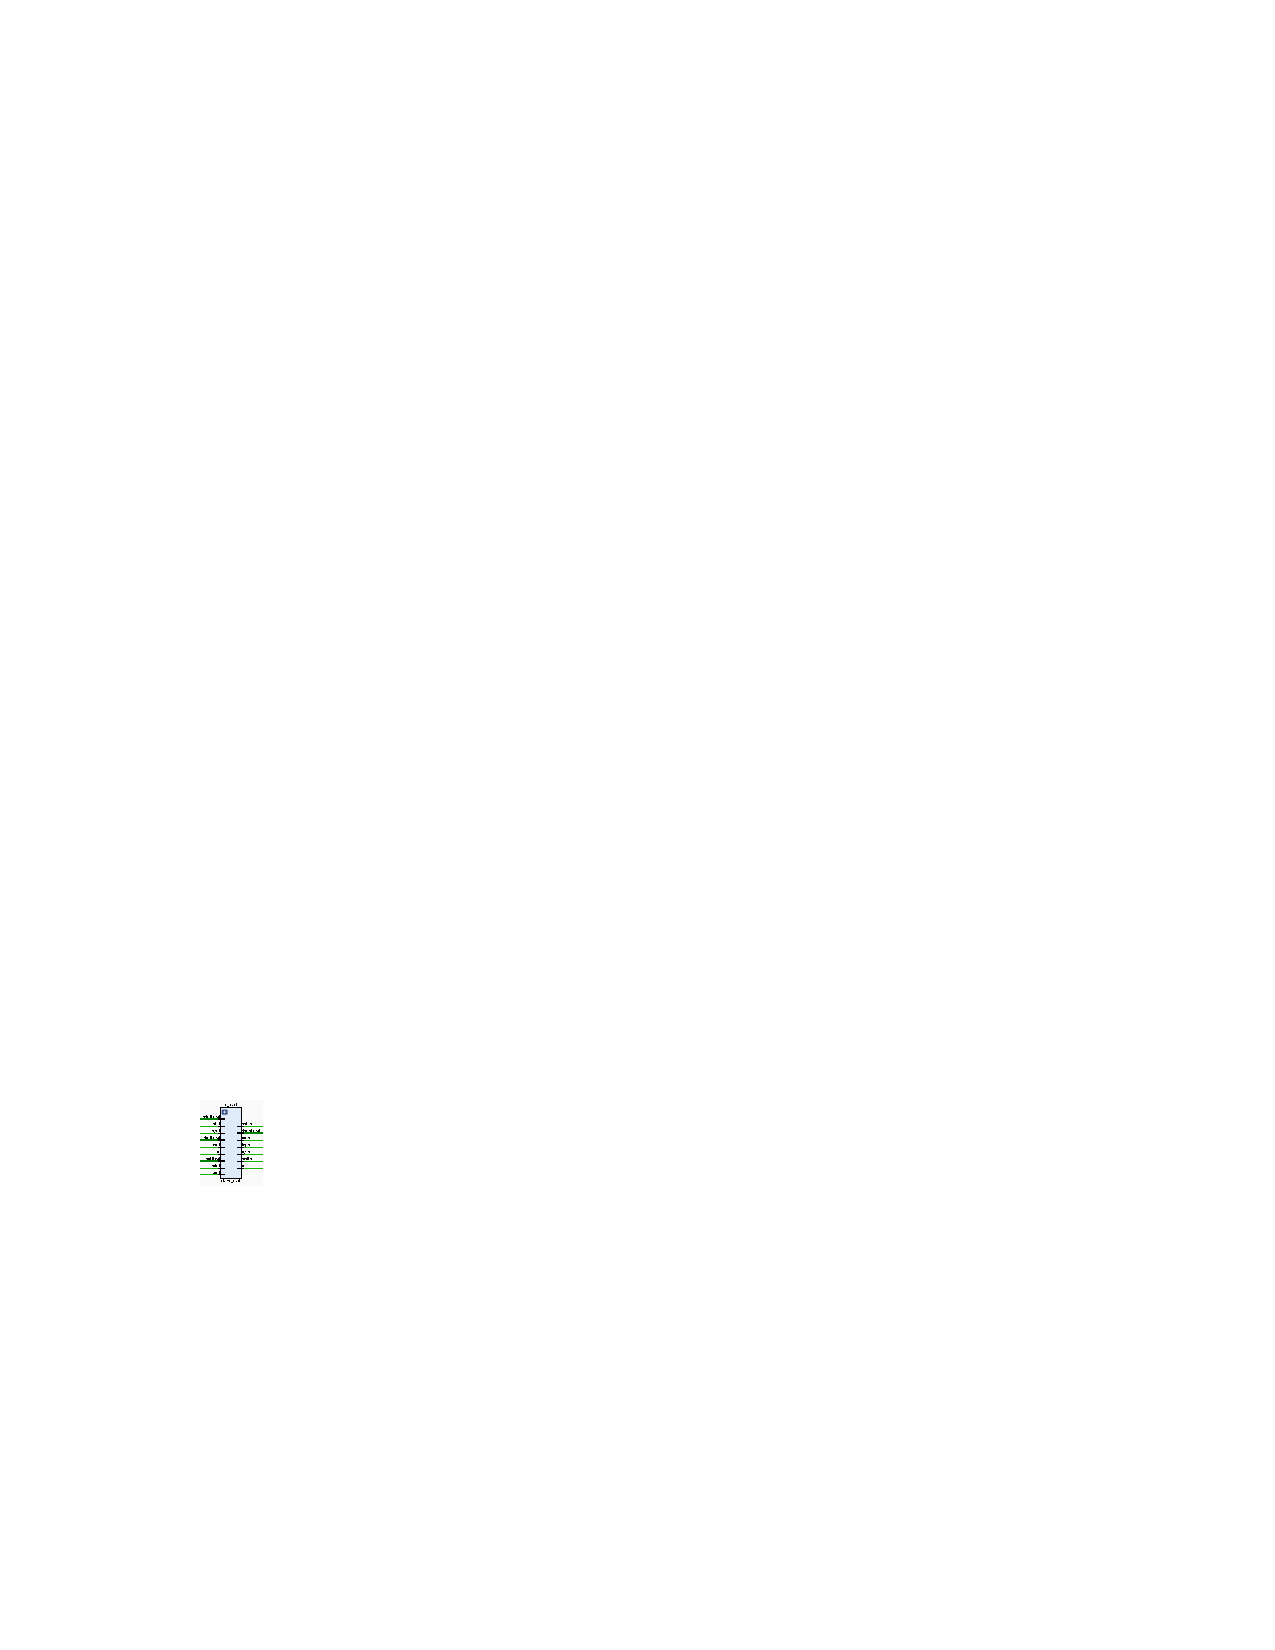
\includegraphics[width=0.3\linewidth]{images/uart}
	\caption{Schaltplanausschnitt: UART}
	\label{fig:shared_bus_uart_sch}
\end{figure}

Als Basis wurde vorerst der bereits vorhandene UART-Controller aus dem Plasma-Projekt genommen. Dieser sollte in Zukunft gegen eine bessere Komponente ausgetauscht werden. Die abgeleitete UART-Frequenz ist von der fest konfigurierten Systemfrequenz von \SI{50}{\mega\hertz} abhängig. Problematisch war auch der \enquote{Dauer-Interrupt} dieser Komponente. Hierzu musste auch der Interrupt-Handler umgeschrieben werden, Näheres dazu im \cref{cha:kebabos}.

\begin{table}[!htbp]
	\bigskip
	\centering
	\begin{tabular}{  l | r | r | l }
		\textbf{REGISTER} & \textbf{Adresse} & \textbf{Modus} & \textbf{Beschreibung} \\
		\hline
		control & 0x00 & r/w & control register \\
		status & 0x04 & r/w & status register \\
		data & 0x08 & r/w & data register (UART RX/TX) \\
		\hline		
		\textbf{CONTROL-Register} & \textbf{Bit} & & \\
		\hline
		reset & 0 & r/w & reset device \\
		enable & 1 & r/w & enable device \\
		\hline		
		\textbf{STATUS-Register} & \textbf{Bit} & & \\
		\hline
		ready & 0 & r & device ready \\
		davail & 1 & r & data available \\
		\hline
	\end{tabular}

	\caption{Registermapping UART}
	\label{tab:uart_reg_map}
\end{table}

\subsection{GPIO}

Es wurde ein einfaches GPIO-Modul entwickelt. 

\begin{figure}[!htbp]
	\centering
	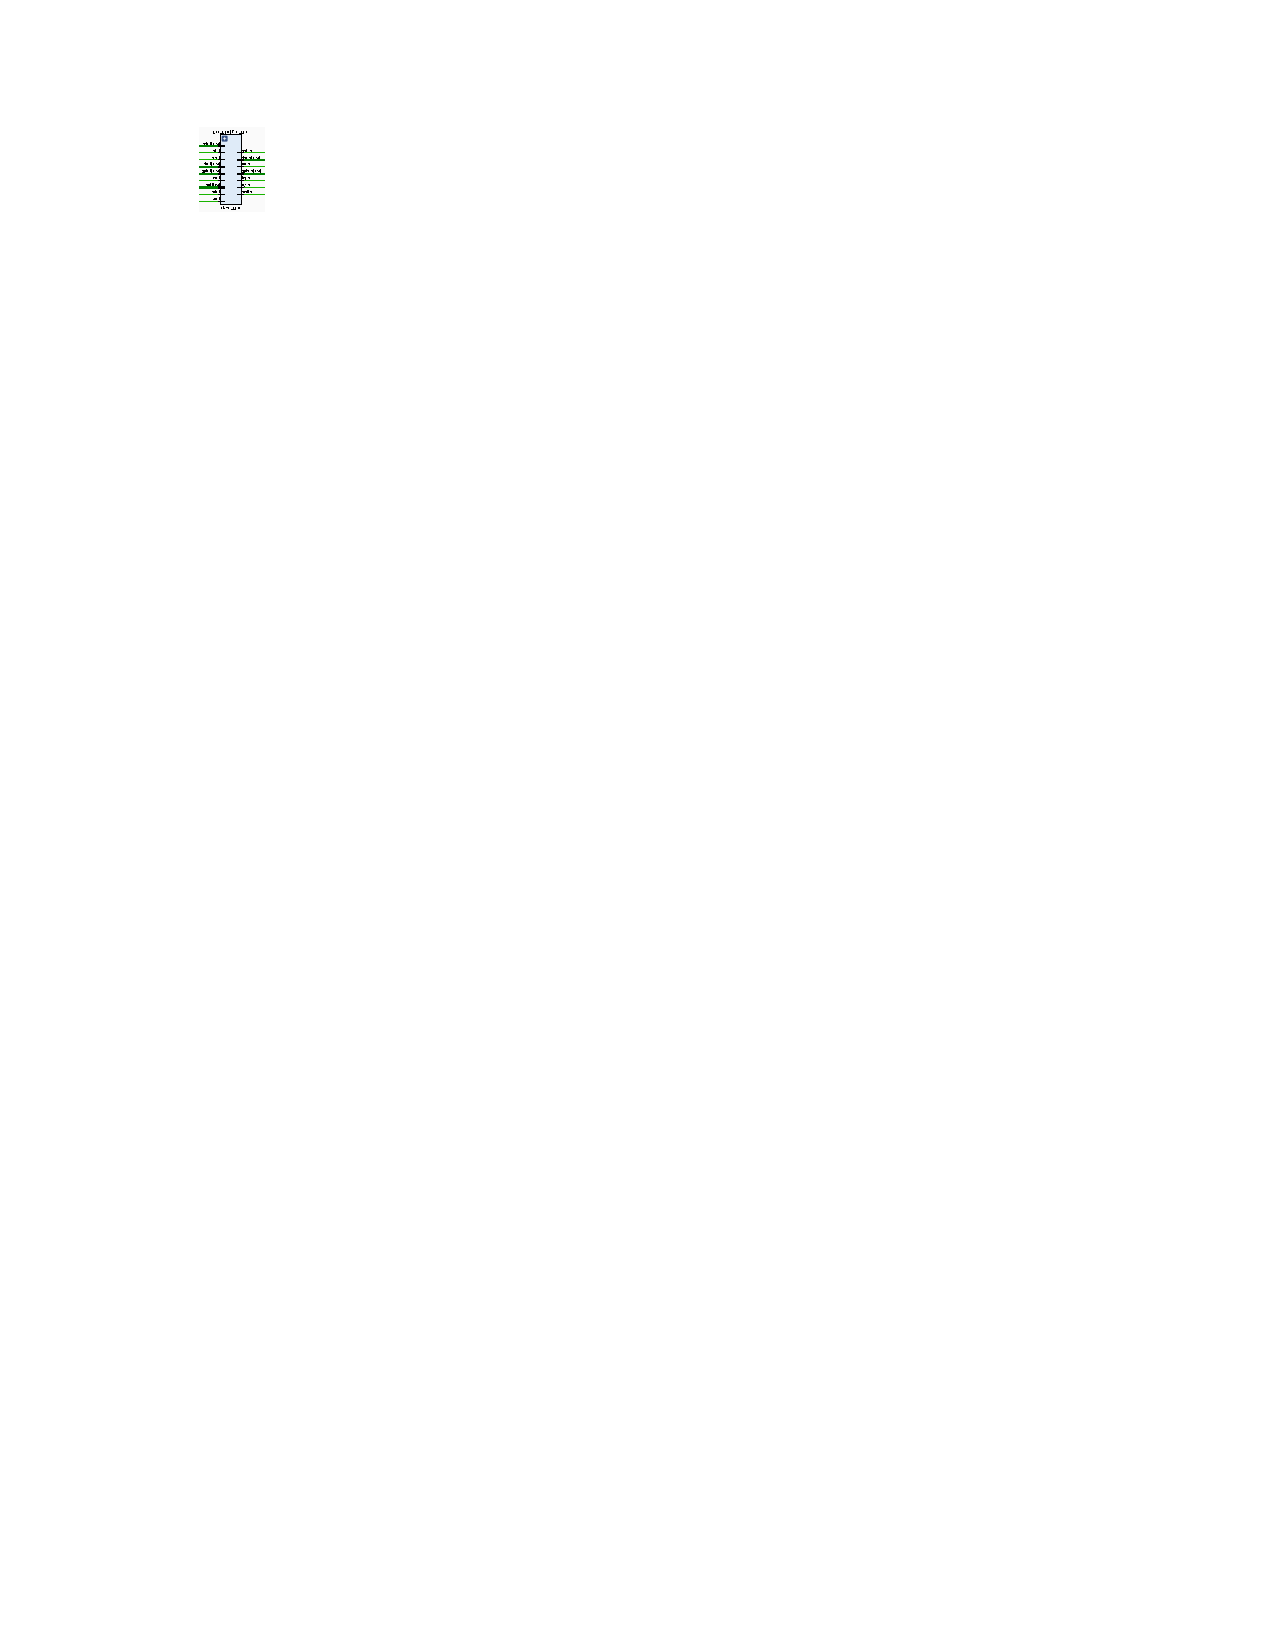
\includegraphics[width=0.3\linewidth]{images/gpio}
	\caption{Schaltplanausschnitt: GPIO}
	\label{fig:shared_bus_gpio_sch}
\end{figure}

\begin{table}[!htbp]
	\bigskip
	\centering
	\begin{tabular}{  l | r | r | l }
		\textbf{REGISTER} & \textbf{Adresse} & \textbf{Modus} & \textbf{Beschreibung} \\
		\hline
		control & 0x00 & r/w & control register \\
		status & 0x04 & r/w & status register \\
		data & 0x0C & r/w & data register (UART RX/TX) \\
		\hline		
		\textbf{CONTROL-Register} & \textbf{Bit} & & \\
		\hline
		reset & 0 & r/w & reset device \\
		enable & 1 & r/w & enable device \\
		\hline		
		\textbf{STATUS-Register} & \textbf{Bit} & & \\
		\hline
		ready & 0 & r & device ready \\
		davail & 1 & r & data available \\
		\hline
	\end{tabular}
	
	\caption{Registermapping GPIO}
	\label{tab:gpio_reg_map}
\end{table}


\subsection{SPI Controller}
\label{ss:spic}

Basierend auf den SPI Controllern aus den \textquote{ZedBoard OLED Display} \cite{website:zedboard_oled} und \textquote{NexysVideo/GPIO} \cite{website:digilent_nexys_video} Projekten wurde ein generischer SPI-Master entwickelt. Konfigurierbar sind die Anzahl Slaves, Datenwortbreite, System- und SPI-Frequenz. Aus der System- und SPI-Frequenz wird der Faktor für den Frequenzteiler gewonnen.

\begin{figure}[!htbp]
	\centering
	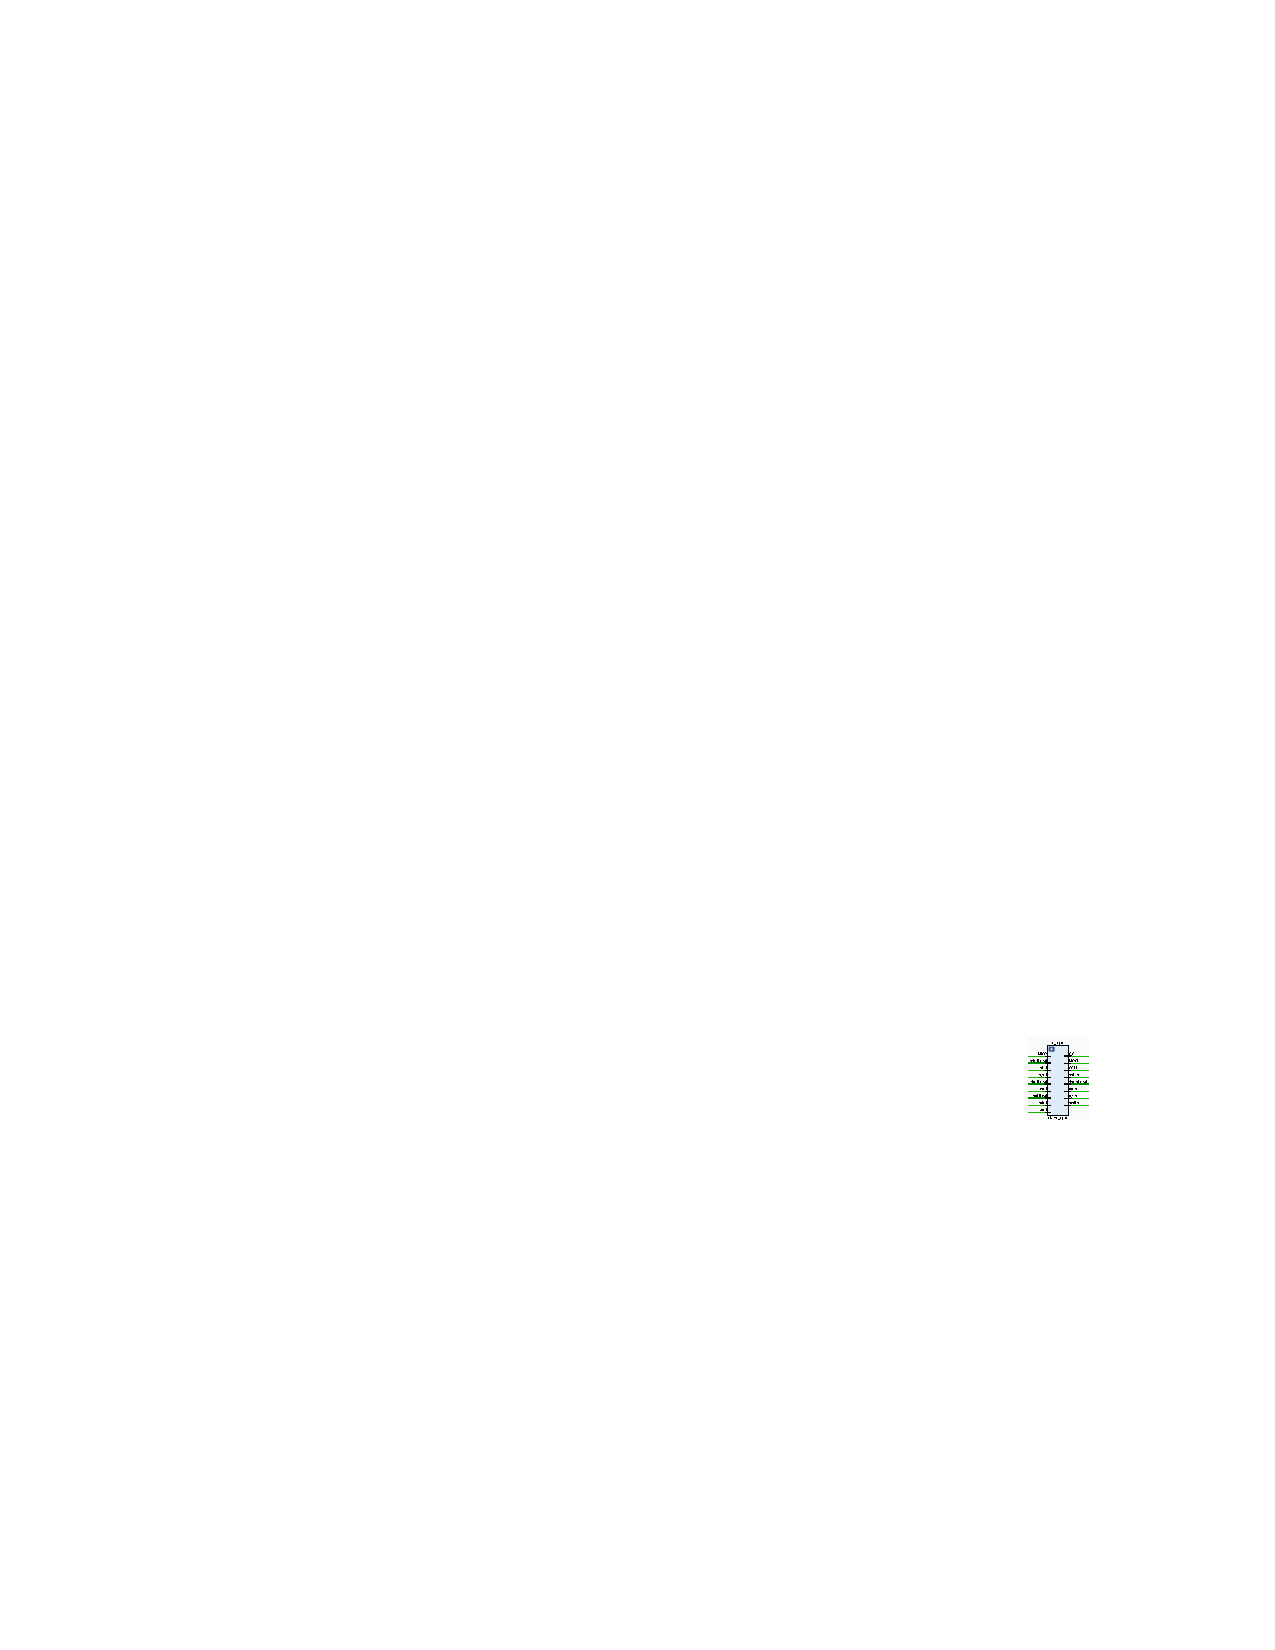
\includegraphics[width=0.3\linewidth]{images/spic}
	\caption{Schaltplanausschnitt: SPI Controller}
	\label{fig:shared_bus_spic_sch}
\end{figure}

\begin{table}[!htbp]
	\bigskip
	\centering
	\begin{tabular}{  l | r | r | l }
		\textbf{REGISTER} & \textbf{Adresse} & \textbf{Modus} & \textbf{Beschreibung} \\
		\hline
		control & 0x00 & r/w & control register \\
		status & 0x04 & r/w & status register \\
		data & 0x08 & r/w & data register  \\
		data & 0x0C & r/w & SPI slave address register  \\
		\hline		
		\textbf{CONTROL-Register} & \textbf{Bit} & & \\
		\hline
		reset & 0 & r/w & reset device \\
		enable & 1 & r/w & enable device \\
		\hline		
		\textbf{STATUS-Register} & \textbf{Bit} & & \\
		\hline
		ready & 0 & r & device ready \\
		davail & 1 & r & data available \\
		\hline
	\end{tabular}
	
	\caption{Registermapping SPI Controller}
	\label{tab:spic_reg_map}
\end{table}

\subsection{OLED Controller}

\begin{figure}[!htbp]
	\centering
	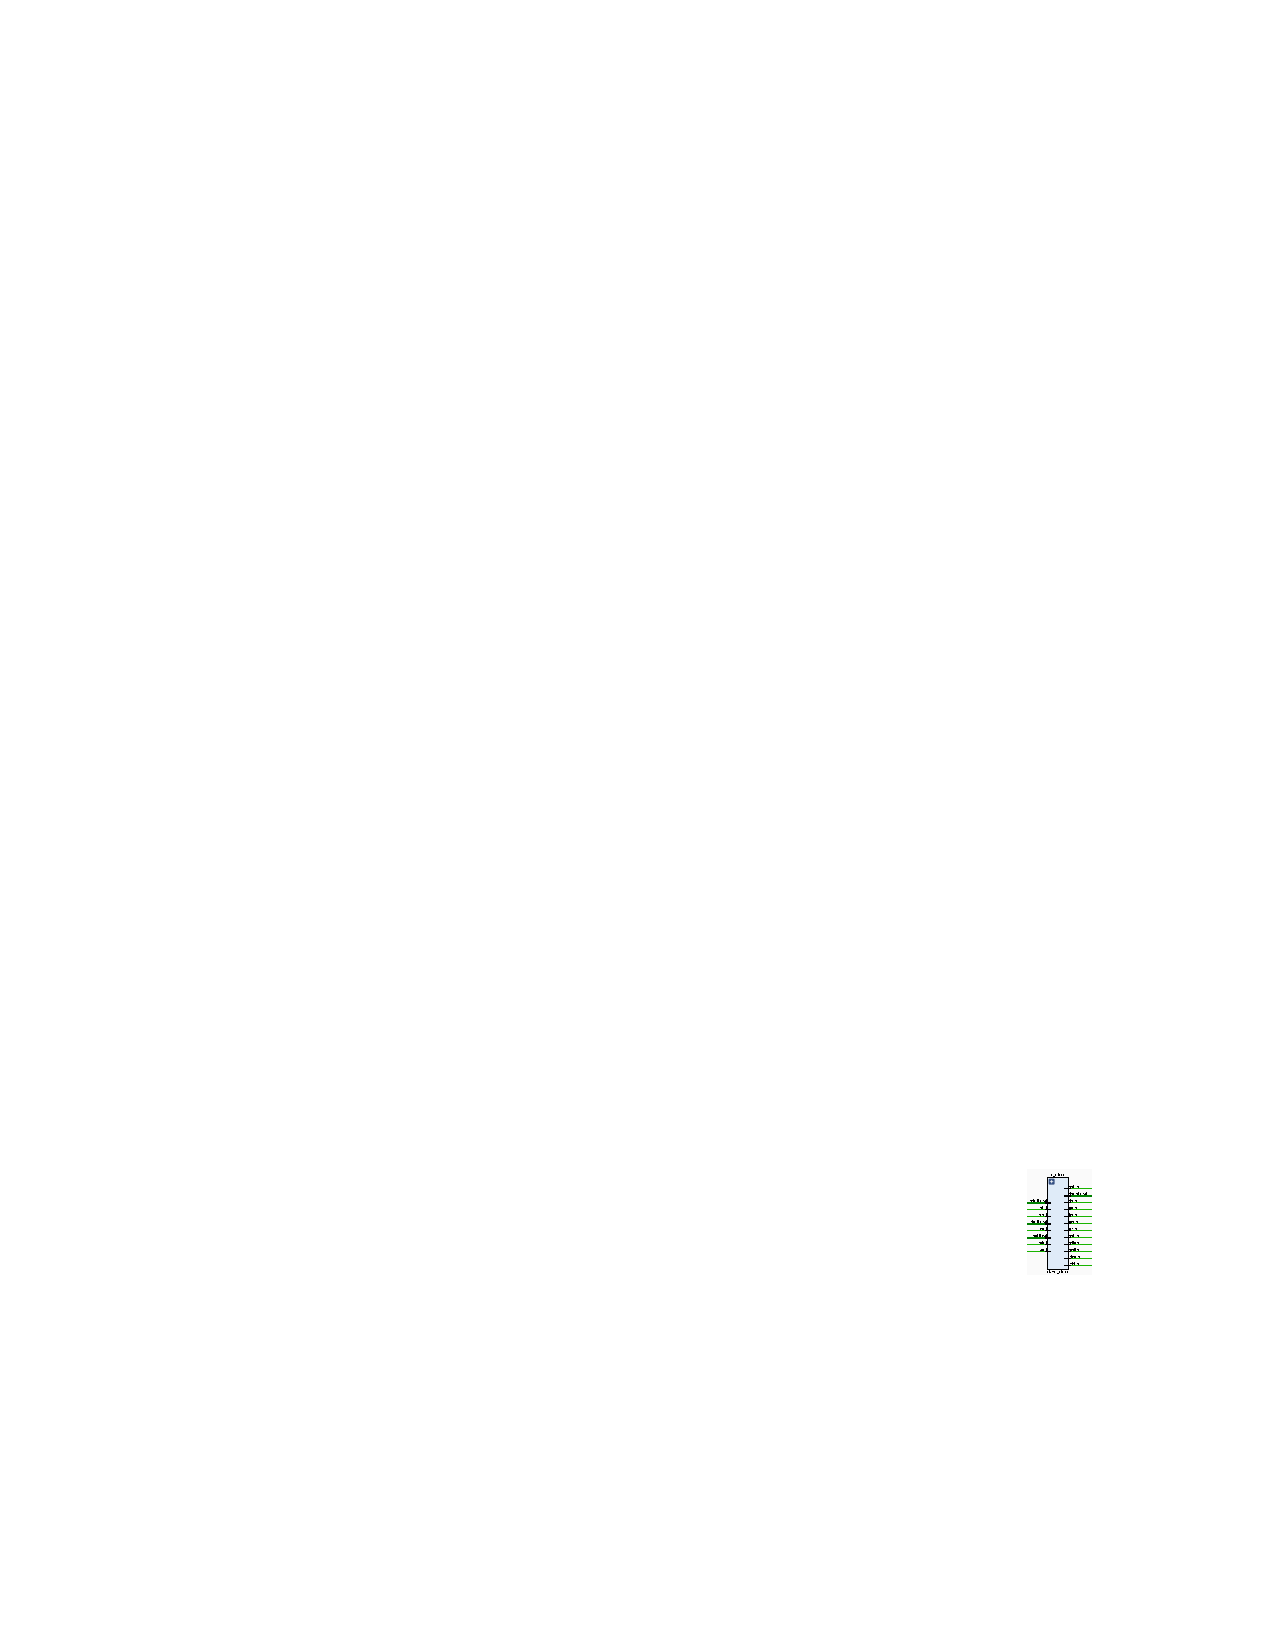
\includegraphics[width=0.3\linewidth]{images/oled_controller}
	\caption{Schaltplanausschnitt: OLED Controller Slave}
	\label{fig:shared_bus_oled_controller_sch}
\end{figure}

Das Display mit der Modellnummer  \textit{UG-2832HSWEG04} wird von Inteltronic/Wisechip hergestellt. Eine  \SI{128 x 32}{\pixel} große, monochrome, passive Matrix steht zur Verfügung. Das Display ist \SI{30 x 11.5 x 1.45}{\milli\meter} groß. \cite[18]{manual:zedboard}

Aufbauend auf Michael Mattioli's Projekt \textquote{ZedBoard OLED Display} \cite{website:zedboard_oled} wurde der Display-Controller entwickelt. Aus der Vorlage wurde die Initialisierungs-, Betriebs- und Beispiellogik, sowie der ASCII-ROM übernommen. Statt des mitgelieferten SPI-Controllers wurde ein eigener Controller (siehe \cref{ss:spic}) verwendet, die Delay-Komponente wurde durch den bereits entwickelten Timer (in \cref{ss:timer} beschrieben) ersetzt. Der Display-Controller unterstützt derzeit nur den Textmodus, d.h der Inhalt des VRAM wird als ASCII-Zeichen interpretiert. Eine Erweiterung um den Grafikmodus ist der Zukunft vorbehalten. Der Immediate-Modus ist dazu vorgesehen, unmittelbar vom Treiber oder Anwendersoftware Befehle bzw. Daten an das Display zu senden, wurde allerdings nicht getestet. Weitere Details sind der Registerzuordnung in \cref{tab:oled_controller_reg_map} zu entnehmen.

\bigskip
\begin{table}[!htbp]
	\bigskip
	\centering
	\begin{tabular}{  l | r | r | l }
		\textbf{REGISTER} & \textbf{Adresse} & \textbf{Modus} & \textbf{Beschreibung} \\
		\hline
		control & \texttt{0x00} & r/w & control register \\
		status & \texttt{0x04} & r/w & status register \\
		data & \texttt{0x08-0x208}  & r/w & vram \\
		\hline		
		\textbf{CONTROL-Register} & \textbf{Bit} & & \\
		\hline
		reset & \texttt{0} & r/w & reset device \\
		enable & \texttt{1} & r/w & enable device \\
		immediate & \texttt{2} & r/w & immediate mode (immediate SPI commands)\\
		textmode & \texttt{3} & r/w & text mode (interpret vram as ASCII chars) \\
		flush & \texttt{4} & r/w & flush vram to screen \\
		clear & \texttt{5} & r/w & clear screen \\
		\hline		
		\textbf{STATUS-Register} & \textbf{Bit} & & \\
		\hline
		ready & \texttt{0} & r & device ready \\
		\hline
	\end{tabular}
	
	\caption{Registermapping OLED Controller}
	\label{tab:oled_controller_reg_map}
\end{table}

\alertwarning{Das Display kann nach dem Board-Start durchaus in einen ungültigen Zustand geraten, sodass, wie in \cref{fig:oled_init_bug} dargestellt, ein Rauschen zu sehen ist. Das ist nicht weiter kritisch, es reicht aus ein Reset auszuführen. Danach ist eine korrekte Funktion sichergestellt. \cite[11]{manual:univision_display}}

\begin{figure}[!htbp]
	\centering
	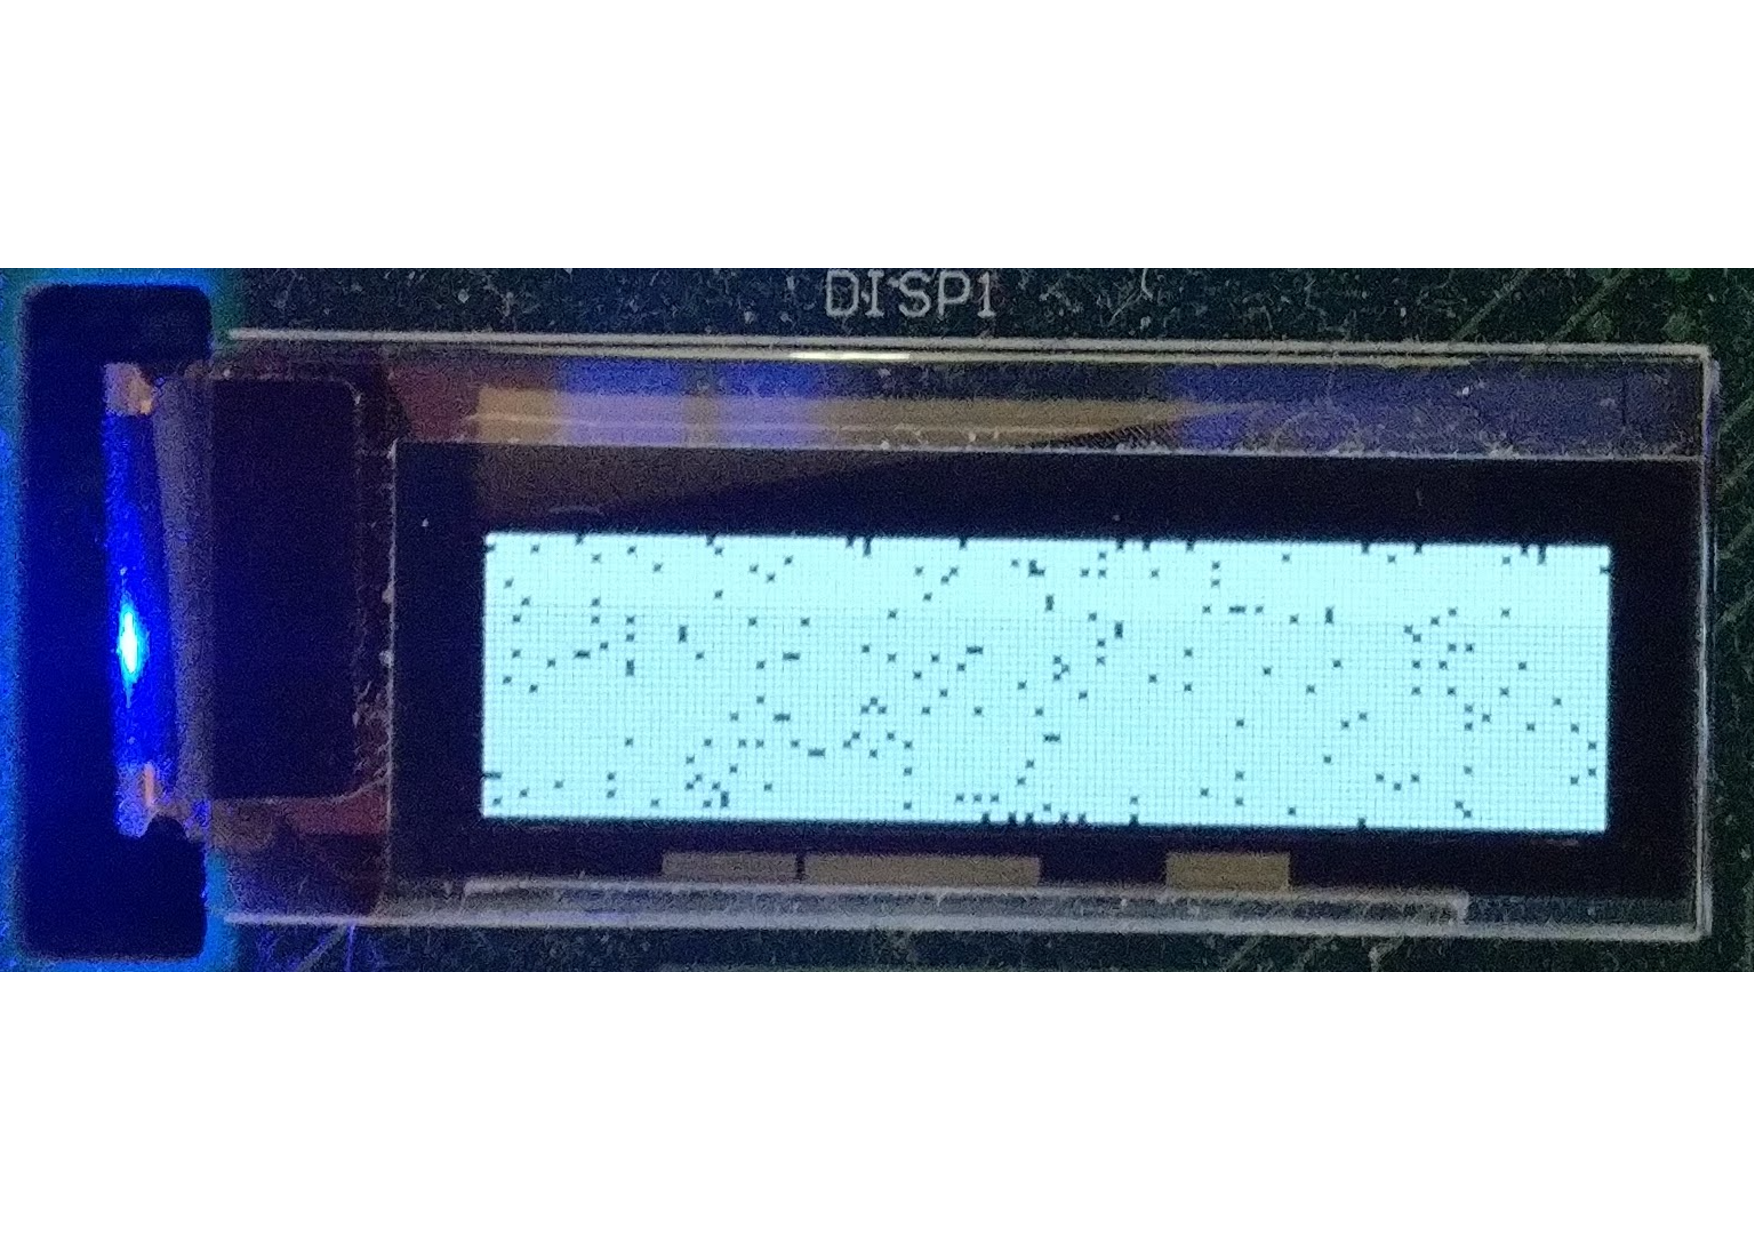
\includegraphics[width=0.3\linewidth]{images/oled_init_bug}
	\caption{Initialisierungsfehler}
	\label{fig:oled_init_bug}
\end{figure}

Der Display-Controller wurde zunächst als ein eigenes Top-Modul auf dem Zedboard getestet, bevor er an das Plasma-SoC angebunden und um Treiber versehen wurde. Die Beispiel-Screens sind in \cref{fig:oled_examples} zu sehen.

\begin{figure}[!htbp]
	\centering
	\begin{subfigure}{.5\textwidth}
		\centering
		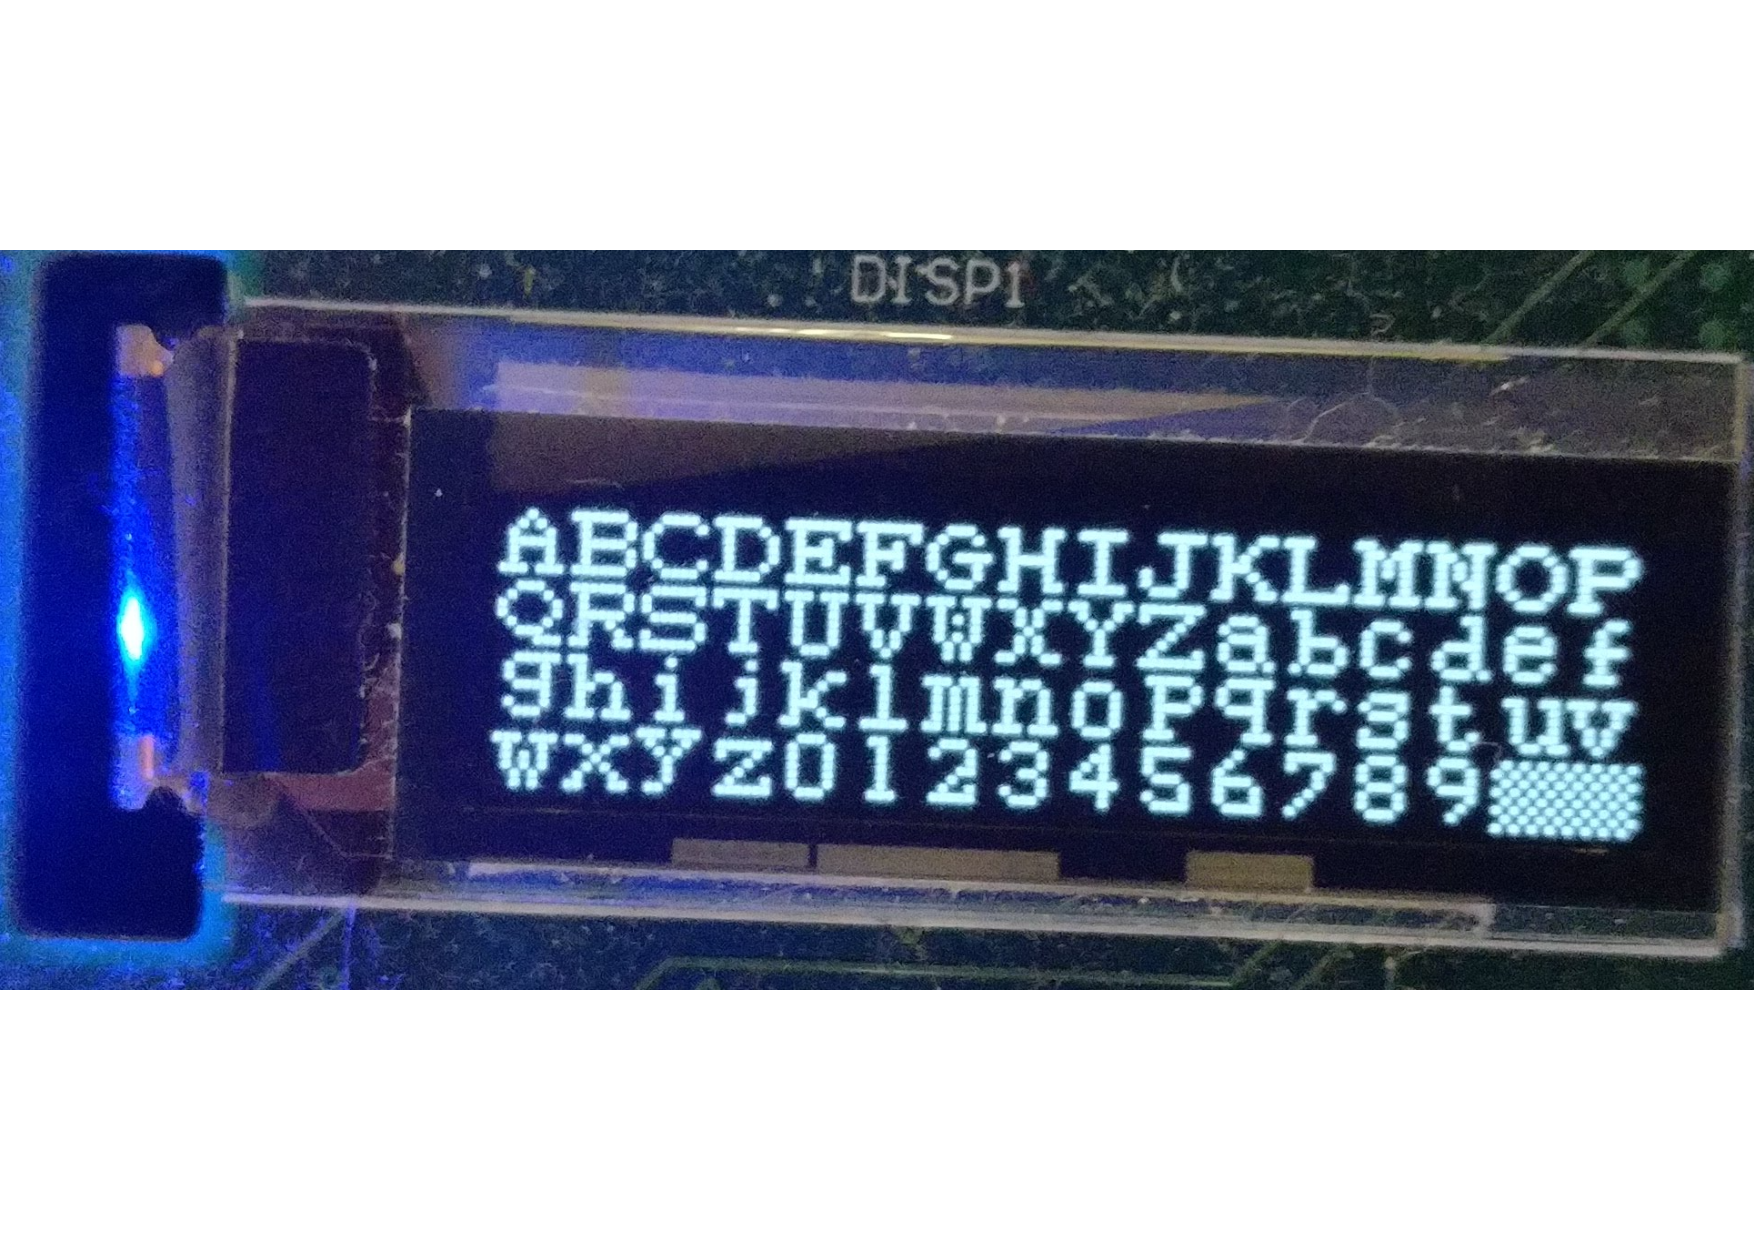
\includegraphics[width=.9\linewidth]{images/oled_char_test}
		\caption{Zeichenfüllung}
		\label{fig:oled_char_test}
	\end{subfigure}%
	\begin{subfigure}{.5\textwidth}
		\centering
		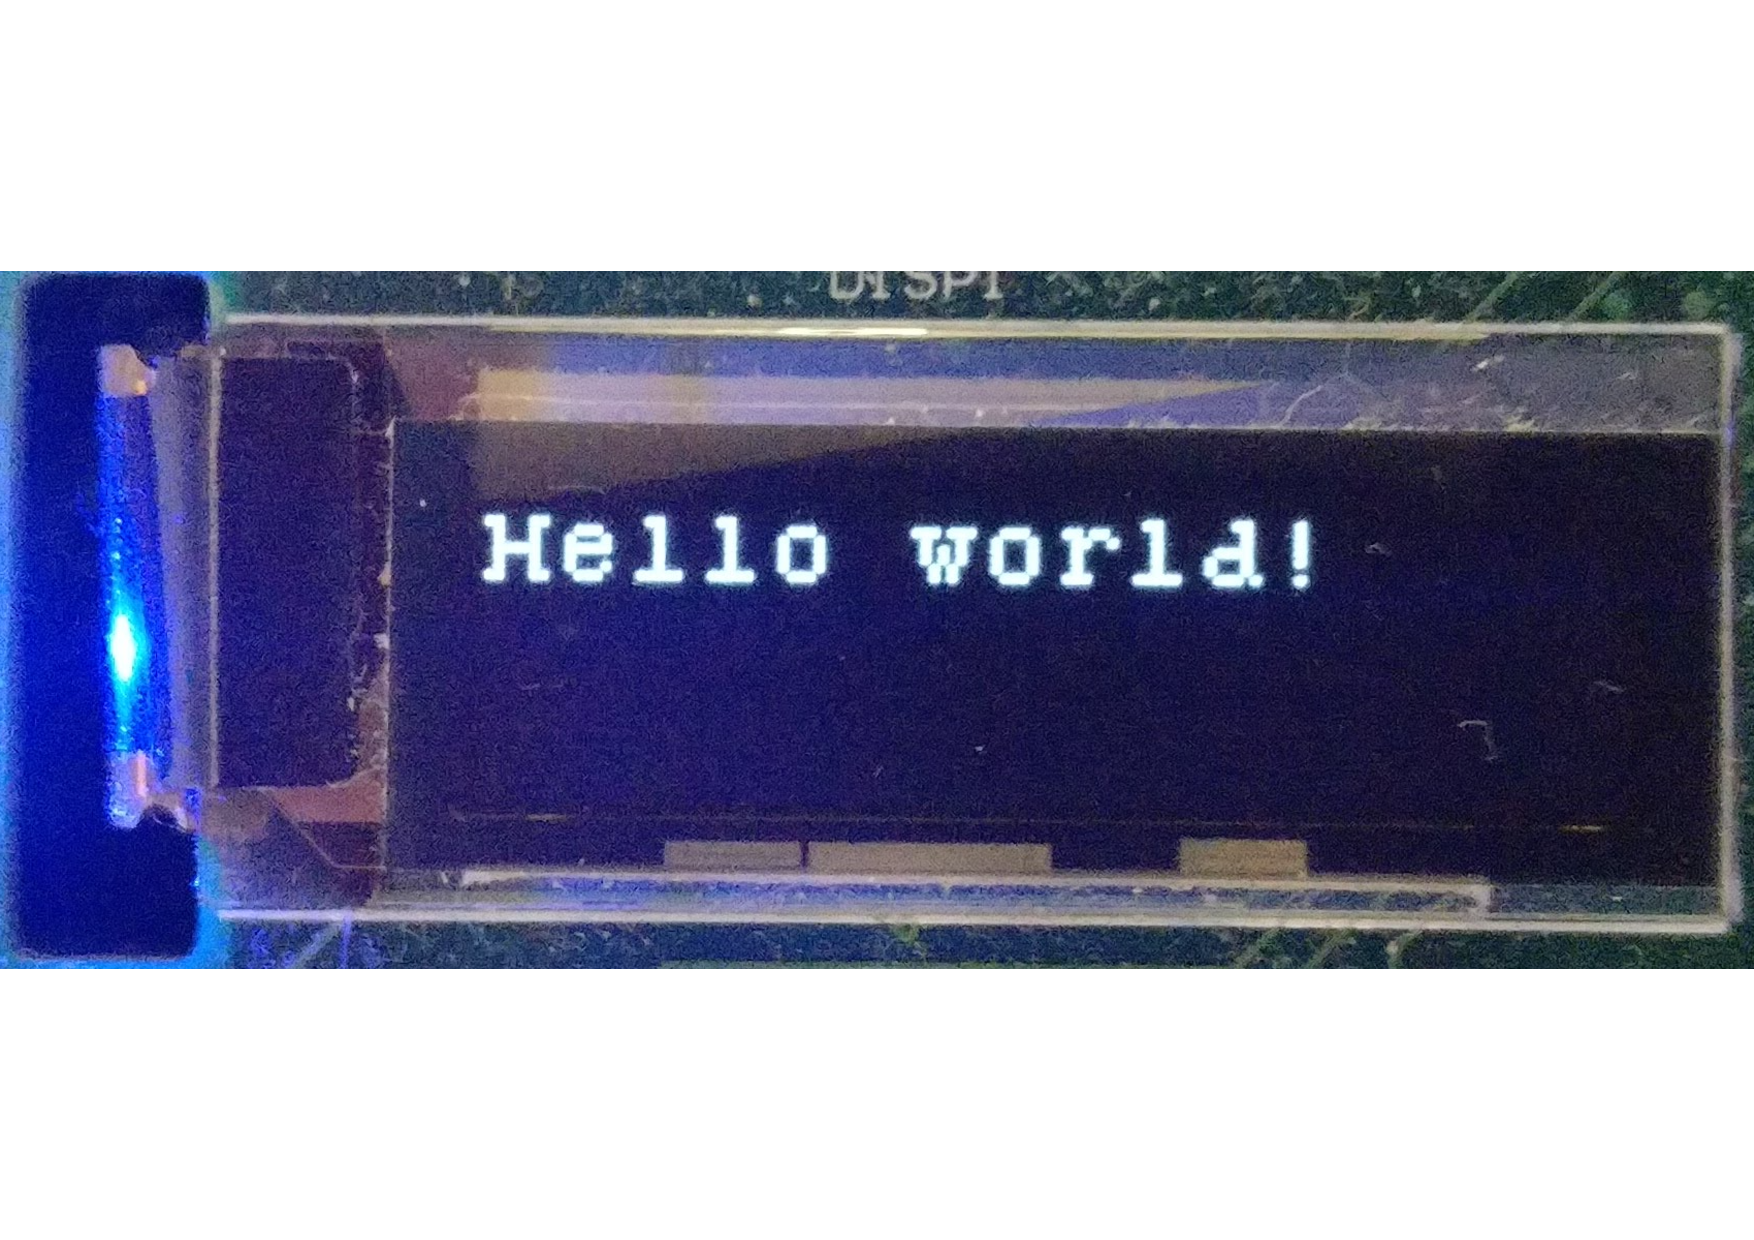
\includegraphics[width=.9\linewidth]{images/oled_hello_world}
		\caption{Hello-World}
		\label{fig:oled_hello_world}
	\end{subfigure}
	\caption{Hardware-Beispiele}
	\label{fig:oled_examples}
\end{figure}

\section{Integration}

Um die in \cref{sec:plasma_soc_components} beschriebenen Komponenten zu einem \gls{SoC} zusammenzuführen, bedarf es einer \gls{Interconnect}-Komponente sowie eines Arbiters. 

%\subsection{Interconnect}

\begin{figure}[!htbp]
	\centering
	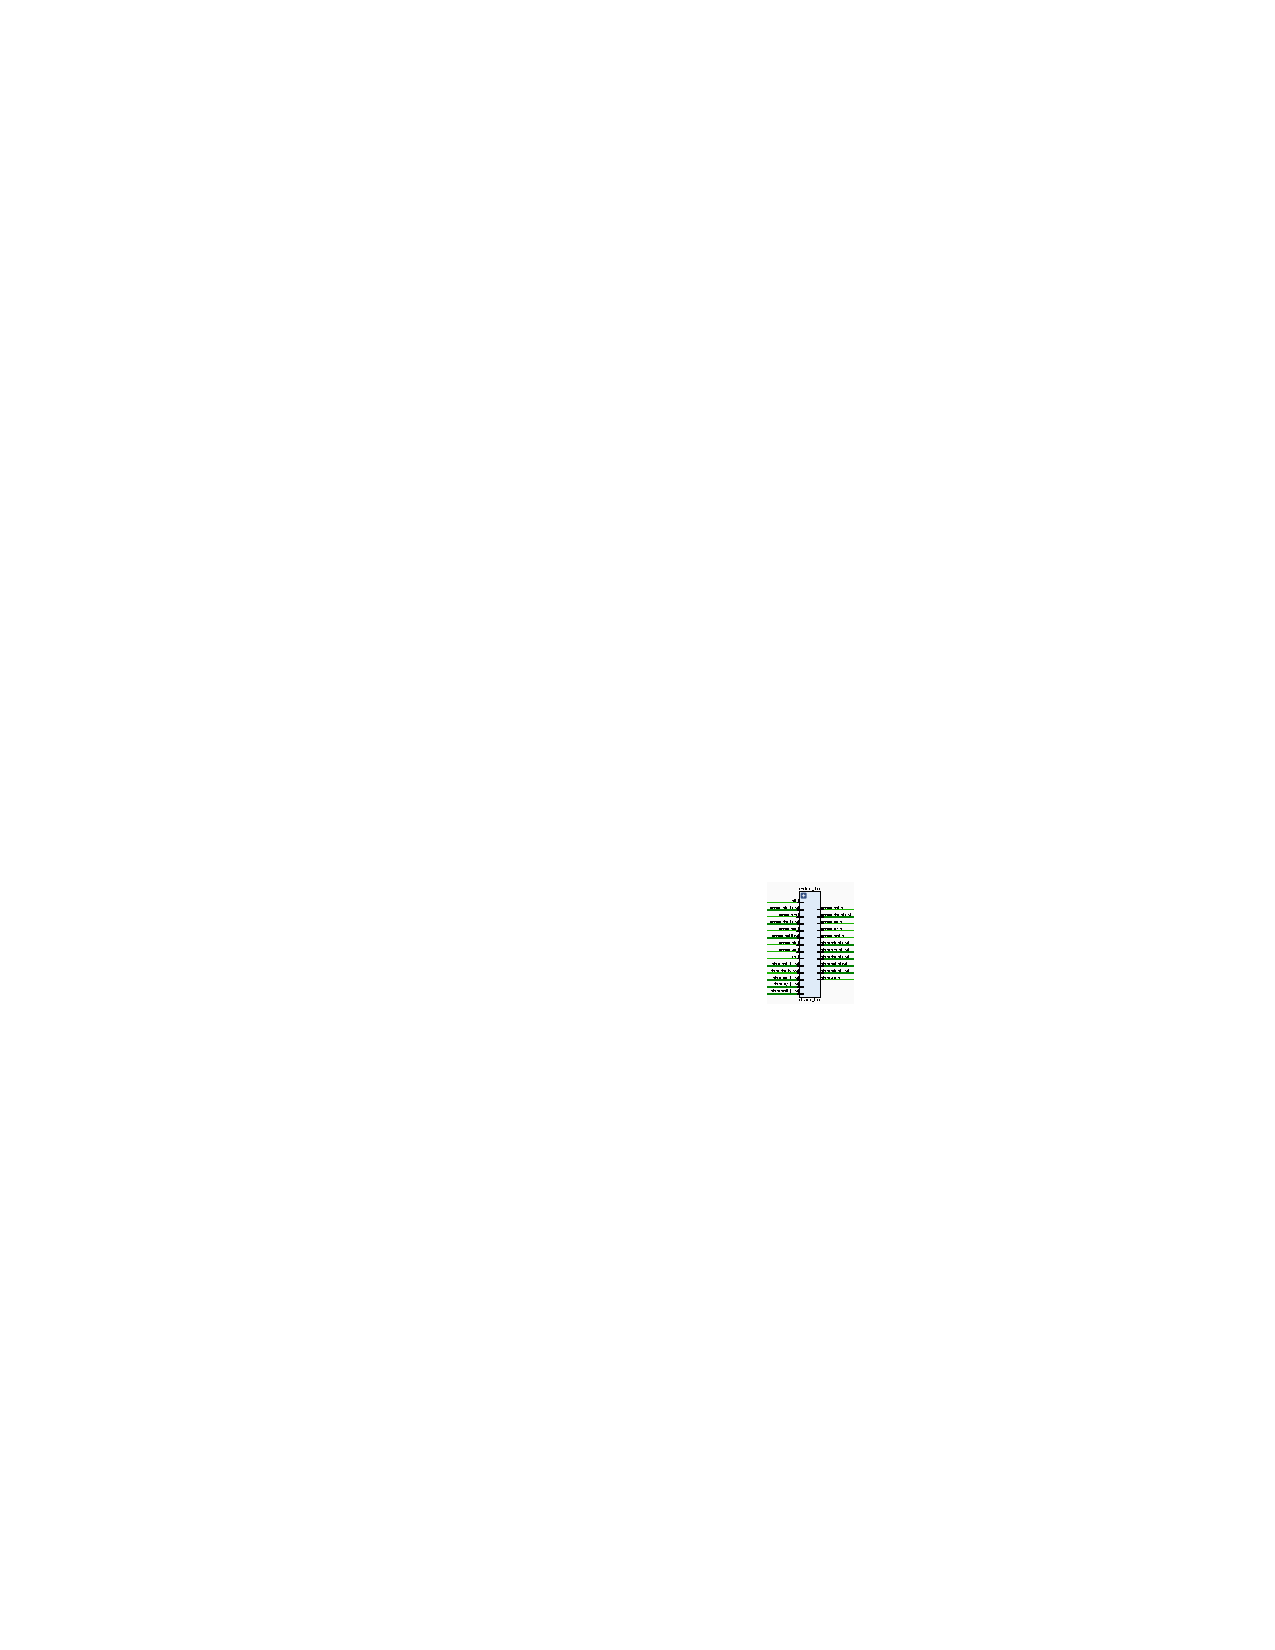
\includegraphics[width=0.3\linewidth]{images/system_bus}
	\caption{Schaltplanausschnitt: Shared bus, 1 Master, 18 Slaves}
	\label{fig:shared_bus_intercon_sch}
\end{figure}

Gemäß der Wishbone-Spezifikation \cites[21]{website:wishbone_b4_spec} wurde der Shared-Bus (Shared-Bus-Topologie) entwickelt. Als Basis für Anspassungen diente das \enquote{boschmitt/wishbone}\cite{website:boschmitt_wishbone} Projekt. Der Bus ist synchron, unterstützt Multi-Master-Betrieb und partielle Adressdekodierung \cite[2]{website:partial_adress_decoding}. Der Bus verwendet keine Tristate-Buffer, sondern ist gänzlich aus Multiplexern aufgebaut. Split transactions \cite[694]{book:computer_architecture} werden nicht unterstützt.
Sollte eine Adresse außerhalb des gültigen (gemappten) Bereiches angesprochen werden, so signalisiert der Bus einen Busfehler. Ein Fehler wird ebenfalls signalisiert, wenn ein Device nach der partiellen Adressdekodierung zwar selektiert, aber ein ungültiges Register angesprochen wird. Um einen Busfehler an den Kernel weiterzugeben, wird der Interrupt 31 verwendet.

%\subsection{Arbiter}

\begin{figure}[!htbp]
	\centering
	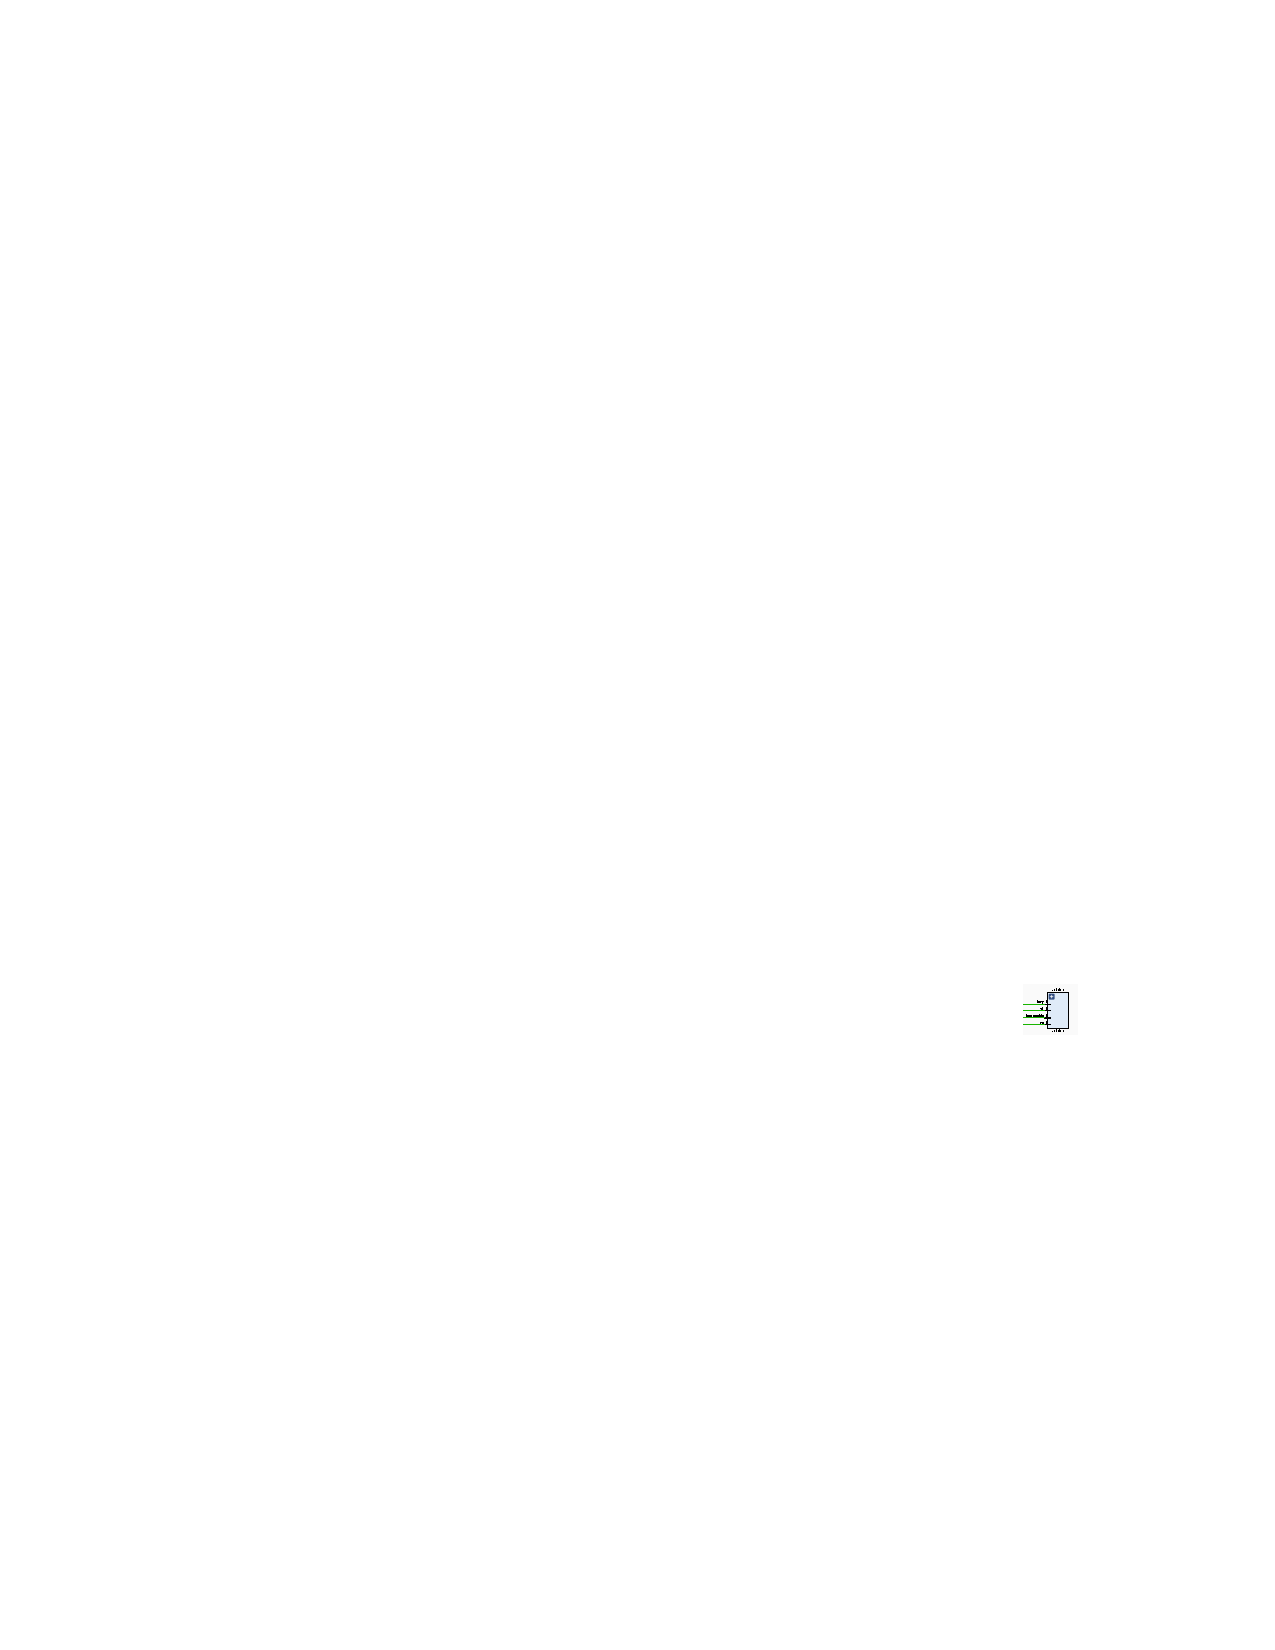
\includegraphics[width=0.3\linewidth]{images/arbiter}
	\caption{Schaltplanausschnitt: Arbiter}
	\label{fig:shared_bus_arbiter_sch}
\end{figure}

Der entwickelte Arbiter arbeitet nach dem priorisiertem Round-Robin-Verfahren: Die Priorität gibt die Anzahl der Zyklen an, für die ein Kanal ausgewählt wird. Ein Kanal kann zudem zur Laufzeit als \textit{ununterbrechbar} markiert werden. Dies ist zum Beispiel für einen Hardware-Boot-ROM vonnützen, um den RAM ununterbrochen zu initialisieren.

Die Anbindung der Komponenten an den Bus erfolgt in der Datei \textit{plasma{\textunderscore}soc.vhd}. Dort werden der Bus und die Komponenten instanziiert, Portdefinitionen sowie die Adresszuordnung erstellt und die Verdrahtung vorgenommen. Die Adresszuordnung ist in \cref{tab:address_map} dargestellt.

\alertwarning{Um die Anzahl der Komponenten zu ändern, müssen die Konstanten \texttt{masters} und \texttt{slaves} sowohl in \textit{plasma{\textunderscore}soc.vhd} als auch in \textit{wb{\textunderscore}pkg.vhd} angepasst werden. Eine Möglichkeit, diesen Verwaltungsaufwand zu umgehen, bieten generische Packages \cite[36-43]{article:vhdl_2008_new_stuff}. Diese sind erst ab VHDL-2008 verfügbar und werden vom Xilinx-Simulator derzeit nicht unterstützt.}

\begin{table}[!htbp]
	\bigskip
	\centering
	\begin{tabular}{ l | r | r }
		\textbf{Gerät} & \textbf{Startadresse} & \textbf{Adressbereich} \\
		\hline		
		Interner \gls{RAM} & \texttt{0x00000000} & \texttt{0x0FFFFFFF} \\
		Externer \gls{RAM} & \texttt{0x10000000} & \texttt{0x001FFFFF} \\
		\hline		
		IRC\textsubscript{0} & \texttt{0x20000000} & \texttt{0x1F} \\
		\hline		
		UART\textsubscript{0}& \texttt{0x00000000} & \texttt{0x0F} \\
		\hline
		\multirow{4}{*}{Timer\textsubscript{0:3}} & \texttt{0x20000200} & \texttt{0x0F} \\
		& \texttt{0x20000210} & \texttt{0x0F} \\
		& \texttt{0x20000220} & \texttt{0x0F} \\
		& \texttt{0x20000230} & \texttt{0x0F} \\
		\hline
		\multirow{4}{*}{Zähler\textsubscript{0:3}} & \texttt{0x20000300} & \texttt{0x0F} \\
		& \texttt{0x20000310} & \texttt{0x0F} \\
		& \texttt{0x20000320} & \texttt{0x0F} \\
		& \texttt{0x20000330} & \texttt{0x0F} \\
		\hline
		\multirow{4}{*}{GPIO\textsubscript{0:3}}  & \texttt{0x20000400} & \texttt{0x0F} \\
		& \texttt{0x20000410} & \texttt{0x0F} \\
		& \texttt{0x20000420} & \texttt{0x0F} \\
		& \texttt{0x20000430} & \texttt{0x0F} \\
		\hline
		SPI\textsubscript{0} & \texttt{0x20000500} & \texttt{0x0F} \\
		\hline
		OLED & \texttt{0x40000000} & \texttt{0x7F} \\
		\hline
	\end{tabular}
	
	\caption{Adresszuordnung}
	\label{tab:address_map}
\end{table}

Für sämtliche Komponenten wurden Interrupts definiert. Da der neue Interrupt-Controller mit 32 Kanälen parametrisiert ist, kann man 32 verschiedene \glspl{IRQ} definieren. Diese sind in \cref{tab:interrupts} aufgelistet. Dabei sind die \glspl{IRQ} 30 bis 15 nicht zugeordnet und für künftige Erweiterungen gedacht.

\begin{table}[!htbp]
	\bigskip
	\centering
	\begin{tabular}{ l | c | c | c | c | c | c | c | c }
		\textbf{\gls{IRQ}} & 31 & 30:15 & 14 & 13:10 & 9:6 & 5:2 & 1 & 0 \\
		\hline
		& Busfehler & $\emptyset$ & OLED & GPIO\textsubscript{3:0} & Zähler\textsubscript{3:0} & Timer\textsubscript{3:0} & UART\textsubscript{w} & UART\textsubscript{r} \\
		\hline
	\end{tabular}
	
	\caption{\glspl{IRQ}}
	\label{tab:interrupts}
\end{table}